\documentclass{elsarticle}
\journal{J. Network and Computer Applications}

\biboptions{sort&compress}
\bibliographystyle{alpha}

\usepackage{amsmath,amssymb,amsfonts}
\usepackage{csquotes}
\usepackage{float}
\usepackage{subcaption}

% HASKELL SYNTAX HIGHLIGHTING - MUST BE LOADED BEFORE xcolor and listings IF THEY'RE ALSO BEING USED
\usepackage{mpshaskell}
\newcommand{\code}[1]{\haskell{#1}}
\newTypeName{Tree,Forest}
%\newCodeWord{tree,list,original,reversed,x,xs,f,f',f'',y,ys,tour_x,tour_y,ex,ey,h,h',h'',e,e1,e2}
%\newFunction{empty,singleton,member,reroot,splice,error,select,link,fromList',cut,path,guard,father}
\newFunction{linkTree,cutTree,conn,link,cut,reroot,root}
\newSymbol{\insertL}{\lhd}
\newSymbol{\insertR}{\rhd}
% END OF HASKELL SYNTAX HIGHLIGHTING

\usepackage{xcolor}
\usepackage{graphicx} 
\usepackage{xspace}
\usepackage{url}

% PROOF-READING COMMANDS
\newcommand{\tcr} [1]{\textcolor{red}{#1}}
\newcommand{\tcb} [1]{\emph{\textcolor{blue}{#1}}}
\newcommand{\madd}[1]{\textcolor{Purple}{#1}}
\newcommand{\mdel}[1]{\textcolor{Yellow}{#1}}

% FORMATTING
\newcommand{\MATHSF}[1]{\ensuremath{\mathsf{#1}}\xspace}

% SYNTAX
\newcommand{\link}{\MATHSF{link}}
\newcommand{\cut}{\MATHSF{cut}}
\renewcommand{\root}{\MATHSF{root}}
\newcommand{\reroot}{\MATHSF{reroot}}
\newcommand{\conn}{\MATHSF{conn}}
\newcommand{\dyntset}{\MATHSF{dynTsET}}

% SYMBOLS
\renewcommand{\O}{\ensuremath{\mathcal{O}}}


\begin{document}
\title{Dynamic Trees through Euler Tours\\%
\large{A purely functional programming approach}}

\author{J.C.~Saenz-Carrasco\fnref{conacyt}\corref{cor1}}
\ead{jcsaenzcarrasco1@sheffield.ac.uk}

\author{M.~Stannett}
\ead{m.stannett@sheffield.ac.uk}

\address{Department of Computer Science,\\
Regent Court, 211 Portobello,\\
Sheffield S1 4DP, United Kingdom}

\cortext[cor1]{Corresponding author}
\fntext[conacyt]{Postgraduate research student, supported by the Consejo Nacional de Ciencia y Tecnolog\'{i}a, CONACYT (Mexican National Council for Science and Technology) under grant 411550, scholar 580617, CVU 214885.}

\begin{abstract}
We introduce a novel dynamic data structure which simultaneously supports $\O(\log n)$ amortised complexity for all three of the basic dynamic operations on forests (\link, \cut and \conn), where $n$ is the total number of vertices. While existing functional structures mirror these time bounds in isolation, ours supports all three of the operations within a single structure. To demonstrate that the algorithms perform well in practice we have implemented them in Haskell and conducted various benchmarking experiments. The results support our theoretical analysis, while also pointing the way to remaining inefficiencies ripe for exploration. We discuss these in detail and consider potential next steps.
\end{abstract}

\begin{keyword}
Dynamic tree algorithms \sep functional programming \sep persistent data structures \sep Haskell
\end{keyword}


\maketitle

% 

\tcr{---------- P O S I T I V E    C O M M E N T S ------------------}


\tcr{This paper introduces Euler Tour Finger Trees (ETFTs), a persistent, purely-functional tree and forest data structure that supports O(log n) complexity for all operations, including link and cut. It gives an implementation in Haskell.}

\tcr{At a high-level, the tree is represented as an Euler Tour (a list of vertex pairs describing a path through the tree), which in turn is represented by a finger tree, thereby allowing O(log n) concatenation and splitting. That allows manipulating Euler tours efficiently, and building interesting tree operations easily.}

\tcr{Most of the implementation in this paper thus builds on existing implementations of finger trees and sets. Yet the combination seems novel, and the complexity bounds of the ETFT operations follow almost trivially, which is nice.
The paper presents a functional data structure for maintaining a dynamic forest under link and cut operations. It realizes this in O(log n) time complexity per operation (amortized), using an Euler tour tree representation implemented using a combination of finger trees and sets. }

\tcr{The paper first recalls dynamic trees and their operations, and then monoids, sets implemented with balanced search trees, Euler-tour trees and finger trees. It then gives (graphical) examples of how the sets and finger trees fit together to realize dynamic trees, it recalls graphically the root, reroot, split, concatenation, and view operations of finger trees, and then walks through the implementation of root, reroot, connected, link, and cut.
Finally the paper contains experiments illustrating that the implementation meets the claimed complexity bounds and discusses related and future work.
This is an interesting piece of work.}




\section{Introduction}
\label{sec:Intro}


In this paper we introduce a new data type that supports efficient querying and editing of massive dynamically changing forests, e.g. the forest of component spanning trees in a collection of dynamically changing d-hoc networks, in the context of functional programming. The use of functional programming is to some extent incidental, but the efficiency of our approach certainly relies on aspects of functional programming -- in particular, the use of lazy evaluation.

The importance of choosing the right functional data type has been demonstrated on an application-by-application basis by many authors. For example, Sleator and Tarjan used path-decomposition with \textit{link-cut} trees for solving network flow problems \cite{DS-DynTs}. Frederickson showed how \textit{topology} trees can be used with tree contraction to maintain minimum spanning trees \cite{DSs-Online-Upd-MSTs}. Of particular interest for our purposes are Henzinger and King's \textit{Euler tour} (ET) trees, introduced by them to speed up dynamic connectivity checking on graphs \cite{Rand-DynGs-Algos}. We adopt their \textit{linearisation} approach, in which trees (of any degree) are re-expressed using a flattened sequence-like representation, thereby allowing a non-linear structure to be manipulated as if it were linear.

All the above techniques have been implemented and studied for ephemeral i.e. non-functional) data structures, performing $\O(\log n)$ per operation. Functional data structures, on the other hand, ease the reasoning and implementation for the cases when preserving history is needed as in self-adjusting computation \cite{DynamizingAlgos} or as in version control \cite{CVS-Demaine}. To overcome the lack of pointers, researchers have devised data structures to represent efficient sequences, most notably, \textit{finger trees} \cite{FTs}. This structure performs well, allowing updates and queries in logarithmic time. We introduce the \emph{dynamic trees through Euler-tours}, a variant of the Hinze's and Paterson finger trees, or \dyntset for short. Like the finger tree, the \dyntset edit sequences in logarithmic time while providing dynamic tree operations. The key insight is to make $\O(1)$ steps to perform \textit{connected}, \textit{link}, and \textit{cut} in logarithmic time. In Section \ref{sec:TechDes} we show this for \textit{connected} and \textit{cut}, whereas \textit{link} takes $\O(m \log n)$. In Section \ref{sec:Eval} we show that, in practice, different results can be obtained, such $\O(1)$ per operation as long as \link is interleaved with \cut.
 \tcb{NO FURTHER explanation about the $\O(1)$ performance}


\paragraph{Contribution}
Our contribution in this paper is to provide a novel functional programming data structure for network representation that allows the programming of suitable low-complexity algorithms, and we provide experimental confirmation of our performance claims. Our results both exploit and rely on the properties of finger trees (Hinze and Paterson). We extend the application of finger trees, offer a solution for dynamic connectivity when facing persistent data structures, and provide a simple interface to the user. The \dyntset exposes two types, \code{Tree} and \code{Forest}, to the user. 

Figure \ref{fig:semantics} describes the functions relevant to our investigation. Table \ref{tab:our-complexities} lists their types (expressed in Haskell format) and (amortised) time complexities. In addition to these, we make free use of functions provided by Hinze and Paterson for finger tree manipulation \cite{FTs}.


\begin{figure}[!htb]
\noindent \underline{Tree manipulation}
\begin{itemize}
\item \code{linkTree v1 t1 v2 t2 :: Tree} \\
   adds a new edge linking vertex \code{v1} of tree \code{t1} to vertex \code{v2} of tree \code{t2}, and returns the resulting tree. \madd{What happens if already in the same tree?}
 \item \code{cutTree v1 v2 t :: (Tree,Tree)} \\
   cuts the edge linking vertices \code{v1} and \code{v2} in tree \code{t}, and returns the resulting pair of trees.
\end{itemize}

\noindent \underline{Forest manipulation and querying}
\begin{itemize}
 \item \code{conn v1 v2 f :: Bool} \\
   returns \code{True} if vertices \code{v1} and \code{v2} in forest \code{f} belong to the same tree, and \code{False} otherwise.
 \item \code{link v1 v2 f :: Forest} \\
   if vertices \code{v1} and \code{v2} belong to different trees, this adds the edge \code{(v1,v2)} to the forest, thereby causing the trees containing \code{v1} and \code{v2} to be joined together to form a new tree; if the vertices already belong to the same tree, the operation has no effect. In either case we return the resulting forest.
 \item \code{cut v1 v2 f :: Forest} \\
     if vertices \code{v1} and \code{v2} are connected by an edge, this removes that edge, thereby causing the tree that contains it to be split into two smaller trees; if the vertices are not connected, the operation has no effect. In either case we return the resulting forest.
\end{itemize}

\noindent \underline{Core functions}
\begin{itemize}
 \item \code{reroot t v :: Tree} \\
   reorganises tree \code{t} so that vertex \code{v} is now root, and returns the resulting tree. \madd{If \code{v} is not a vertex in \code{t}, returns \code{t} unchanged. 
 \item \code{root t :: Maybe(Vertex)} \\
   returns \code{Just v} if \code{v} is the root of the tree \code{t}, and \code{Nothing} otherwise (if the tree is non-empty).
\end{itemize}
\caption{Informal semantics of the functions investigated in this paper. The functions split into three blocks: the first contains functions performing dynamic tree operations; the next lists functions used to compute an unbounded, although finite, sequence of dynamic tree operations on forests; the third deal with basic core functionality.}
\label{fig:semantics}
\end{figure}


\begin{small}
\begin{table}
\caption{Amortised time complexity for various dynamic forest-editing operations. In each case, $n$ gives the number of vertices in the first (or only) tree operated upon; for those functions taking two trees as input, $m$ is the number of vertices in the second tree. The result for \link assumes that $m \leq n$ (if not, we can swap the order of the arguments before applying the algorithm).}
 \begin{tabular}{|| l | l | l ||} 
 \hline
 Function & Type & Time complexity \\ %[0.5ex] 
 \hline\hline
 \texttt{linkTree} & \texttt{Vertex} $\to$ \texttt{Tree} $\to$ \texttt{Vertex} $\to$ \texttt{Tree} $\to$ \texttt{Tree} & $\O(m\log n)$ \\
 \texttt{cutTree} & \texttt{Vertex} $\to$ \texttt{Vertex} $\to$ \texttt{Tree} $\to$ \texttt{(Tree,Tree)} & $\O(\log n)$ \\
 \hline
 \texttt{conn} & \texttt{Vertex} $\to$ \texttt{Vertex} $\to$ \texttt{Forest} $\to$ \texttt{Bool} & $\O(\log n)$ \\ 
 \texttt{link} & \texttt{Vertex} $\to$ \texttt{Vertex} $\to$ \texttt{Forest} $\to$ \texttt{Forest} & $\O(m\log n)$ \\
 \texttt{cut} & \texttt{Vertex} $\to$ \texttt{Vertex} $\to$ \texttt{Forest} $\to$ \texttt{Forest} & $\O(\log n)$ \\
 \hline
 \texttt{reroot} & \texttt{Tree} $\to$ \texttt{Vertex} $\to$ \texttt{Tree} & $\O(\log n)$ \\
 \texttt{root} & \texttt{Tree} $\to$ \texttt{Maybe(Vertex)} & $\O(1)$ \\
 \hline   
\end{tabular}
\label{tab:our-complexities}
\end{table}
\end{small} 



\subsection*{Structure of the paper}
In the next section, we give an overview of the finger tree functions and their performance. These are the foundations for our functions altogether with some of the functions from the Hackage library \texttt{Data.Set} \footnote{https://hackage.haskell.org/package/containers-0.5.10.2/docs/Data-Set.html} which mimic the set-like operations over our functions, such as testing membership. 

%In Section~\ref{sec:Example}, we present an in-depth example using the operations mentioned above. In particular, we depict how the \dyntset manages the trees as sequences under the dynamic setting, showing how the \dyntset structure is constructed immutably. 
In Section \ref{sec:TechDes}, we describe our implementation for performing dynamic tree operations with purely data structures, the \dyntset. The following is the address where our source code is hosted and publicly available:
\begin{center}
\url{https://github.com/jcsaenzcarrasco/ETdynTs}
\end{center}

We evaluate \dyntset empirically in Section~\ref{sec:Eval}. In concrete, we plot the results of benchmarking the functions in the first two sections of the table above. Our evaluation demonstrates that \dyntset performs according the function definitions with a constant factor between \conn and \link and \cut. 

%Section~\ref{sec:Discuss} discuss the main reasons we took into account when designing ETFT, with some suggestions for improving the internal vertex annotations. 
In Section~\ref{sec:RelWrk} we suggest potential alternatives for designing dynamic data structures to solve the problem described in the present document. 

Finally, we conclude in Section~\ref{sec:Concl} with a summary of our work.


\tcr{Presentationally I'm missing a better description of the background material. The paper recalls the definition of a monoid, but does not recall the definition of an Euler tour nor give enough detail on finger trees to read as an independent document.} 


%%%% END OF INTRO
%%%% START OF PRELIM


\section{Preliminaries} 
\label{sec:Prelim} 

Our proposal, \dyntset, relies mainly on three structures, a \textit{monoid}, a \textit{set} and a \textit{finger tree}, which are briefly described in the following subsections. 

\subsection{Monoid}

A \textit{monoid} is a triple $(S,\star,e)$, where $S$ is a set, $\star$ is a binary operation, called $product$ and $e$ is an element of $S$, called $unit$, satisfying the following properties:

\begin{enumerate}
\item $e \star x = x = x \star e$, for all $x \in S$ 
\item $x \star (y \star z) = (x \star y) \star z $, for all $x,y,z \in S$.  
\end{enumerate}

The type class Haskell implementation of a monoid we have:
%\begin{verbatim}
\begin{lstlisting}[mathescape]
class Monoid  a where 
   mempty  :: a
   mappend :: a $\to$ a $\to$ a
\end{lstlisting}   
%\end{verbatim}

where the function \code{mempty} represents the element $e$ and the function \code{mappend} represents function $\star$. Detailed information about monoids within the functional programming can be found in \cite{Monoids}, and for the Haskell implementation at \cite{HaskellMonoid}.


\subsection{Set as binary search tree} 

A set, as a data structure, is used here for searching purposes, seen as testing membership within a specific set. Also, we look for incorporating elements into a set in order to increase such set for further look ups. This incorporation, comes in two flavours, either as single insertion or as the set-union operation. Finally, the presence of an empty set, a set with no elements at all, is crucial since it is the $unit$ when a set behaves as monoid. Also, an empty set is a starting point when a forest contains no trees.

Internally, a set is implemented as binary search tree, also called BST. A BST is either a \textit{leaf} (also called a \code{tip}) or a vertex consisting of a \textit{value}, a \textit{left} BST and a \textit{right} BST. The height of the tree determines the time taken to perform every operation onto it, therefore the shorter the height the better, and this is done throughout a \textit{balancing scheme}. The study of BSTs is vast and there are several implementation around. In our case, a \textit{size balanced} and a \textit{pairing hashed} are used. A detailed comparison and benchmarking is outside the scope of the present work.

The following is an snippet of \code{Data.Set} \footnote{https://hackage.haskell.org/package/containers-0.5.10.2/docs/Data-Set.html}
%\begin{verbatim}
\begin{lstlisting}
data Set a    = Bin Size a (Set a) (Set a)
              | Tip
\end{lstlisting}              
%\end{verbatim}

In Table~\ref{tab:Setfuncs} we show the set-functions we have incorporated in \code{dynTsET} from \code{Data.Set}.
\small
\begin{table}[H]
\begin{center}
\begin{tabular}{||l | l | c||} 
 \hline
 Function         & Type                                   & Time complexity            \\ 
 \hline\hline
 \texttt{empty}   & \texttt{Set a}                         & $\O(1)$                     \\ 
 \hline
 \texttt{insert}  & \texttt{a $\to$ Set a $\to$ Set a}     & $\O(\log n)$                \\
 \hline
 \texttt{member}  & \texttt{a $\to$ Set a $\to$ Bool}      & $\O(\log n)$                \\ 
 \hline
 \texttt{union}   & \texttt{Set a $\to$ Set a $\to$ Set a} & $\O(m(\log\frac{n}{m} +1))$ \\
 \hline
\end{tabular}
\caption{Leijen's implementation of \code{Data.Set} \cite{HaskellSet}, based on \cite{ParallelSets}}
\label{tab:Setfuncs} 
\end{center}
where $n$ and $m$ are the sizes of the largest and smallest sets respectively
\end{table}
\normalsize

Functions \code{empty} and \code{union} are, in fact, the monoidal functions \code{mempty} and \code{mappend} respectively. 

\subsection{Euler-tour tree} 
\label{sec:ETt}
Dealing with trees of different degree can be complicated. A simple way to handle and represent trees of any degree is by an Euler tour, that is, a sequence as in \cite{Rand-DynGs-Algos} and \cite{WerneckR-PhD}. To represent a tree $t$, we replace every edge $\langle u,v \rangle$ of $t$ by two arcs $(u,v)$ and $(v,u)$, and add a loop $(v,v)$ to represent each vertex $v$. In this context, a tree $t$ can have at least one, and in general, many Euler tours. The size of an Euler tour \textit{et} of $t$ is $et(t) = v + 2e $, where $v$ is the number of vertices of $t$ and $e$ its number of edges. We can represent an Euler tour in Haskell simply as a list of pairs, such in 

%\begin{verbatim}
\begin{lstlisting}
data EulerTour a = [(a,a)] 
\end{lstlisting}
%\end{verbatim}

By managing the tour with lists, we can perform insertion from the left (head) in $\O(1)$ but remaining operations such insertion from the right, access, cutting, appending and inserting might take $\O(n)$ per operation.
On the other hand, representing tours through finger trees, performance per operation is improved up to $\O(\log n)$ per operation amortised as we explain shortly and in Section~\ref{sec:TechDes}. 

Our representation of $k$-trees through Euler-tour will not close up the tour with the first node as this avoids the uniqueness presence for such a node, as shown in Fig.~\ref{fig:Euler-tour}.

\begin{figure}[H]
\begin{center}
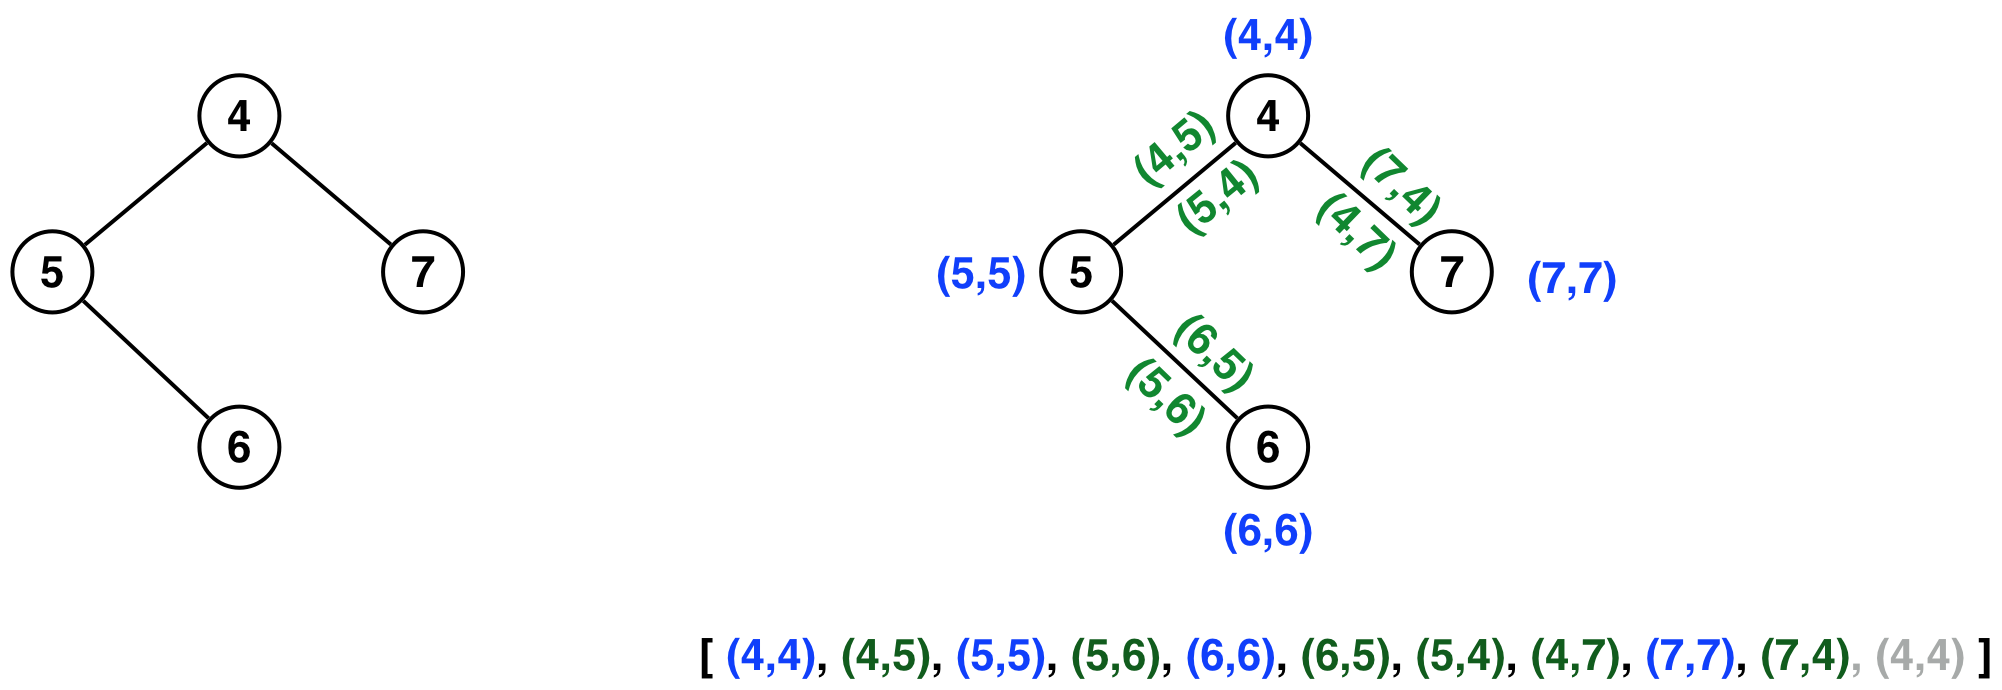
\includegraphics[scale=0.35]{./Images/Euler-tour} 
\end{center}
\caption{The $k$-tree (left) is represented as a sequence of size $v+2e$ (right). Notice we left out the final node-pair to preserve uniqueness}
\label{fig:Euler-tour}
\end{figure}


\subsection{Finger tree} 

We present Hinze and Paterson's version of finger trees \madd{(FTs)} \cite{FTs}. A finger tree is a 2-3-4 tree data structure which is always balanced. The structure is designed to store the elements of a sequence in the terminal nodes or leaves while intermediate nodes are dedicated for monoidal annotations. These annotations help out to achieve a specific task when storing or retrieving values in the leaves or when dealing with the tree itself such concatenation or splitting. One instance is random-access on lists. In order to speed up the time taken by a list for accessing the $n$th element, a finger tree stores the list elements on its leaves and the type \code{Sum Int} as its monoidal annotation. In this way, we can ask for a specific element provided its index in $\O(\log n)$ rather than $\O(n)$ time. This done through monoidal instances for \code{Sum}. The identity is defined as zero as in 
\begin{lstlisting}[mathescape]
instance Num a $\Rightarrow$ Monoid (Sum a) where
        mempty = Sum 0
\end{lstlisting}

and the corresponding binary operation on integers which preserves its identity (arithmetic addition),
\begin{lstlisting}[mathescape]
instance Num a $\Rightarrow$ Semigroup (Sum a) where
        (<>) = coerce ((+) :: a $\to$ a $\to$ a)
\end{lstlisting}


The finger tree data type in Haskell is defined as

\begin{figure}[H]
\begin{lstlisting}
data FingerTree v a = Empty
                    | Single a 
                    | Deep v 
                           Digit a 
                           FingerTree v (Node v a) 
                           Digit a
\end{lstlisting}                           
\caption{Data type of the finger tree by Hinze and Paterson}
\label{fig:FTdatatype}
\end{figure}

\code{Digit} type holds from one up to four elements of type \code{a}. \code{Node} type can hold two or three elements of type \code{a}. The recursive and nested definition of \code{FingerTree} forces the structure to be balanced by its types, instead of enforcing it by code invariants. In our case, the leaves of a finger tree stores pairs of nodes or vertices representing an Euler tour. To implement \textit{updates} and \textit{lookups} efficiently, Hinze and Paterson \cite{FTs} added a monoidal annotation on the intermediate vertices, the \code {v} type.

In Fig.~\ref{fig:FT-Euler-tour} we can see our example of the Euler-tour sequence in Fig.~\ref{fig:Euler-tour} managed by the data constructors described above.

\begin{figure}[H]
\begin{center}
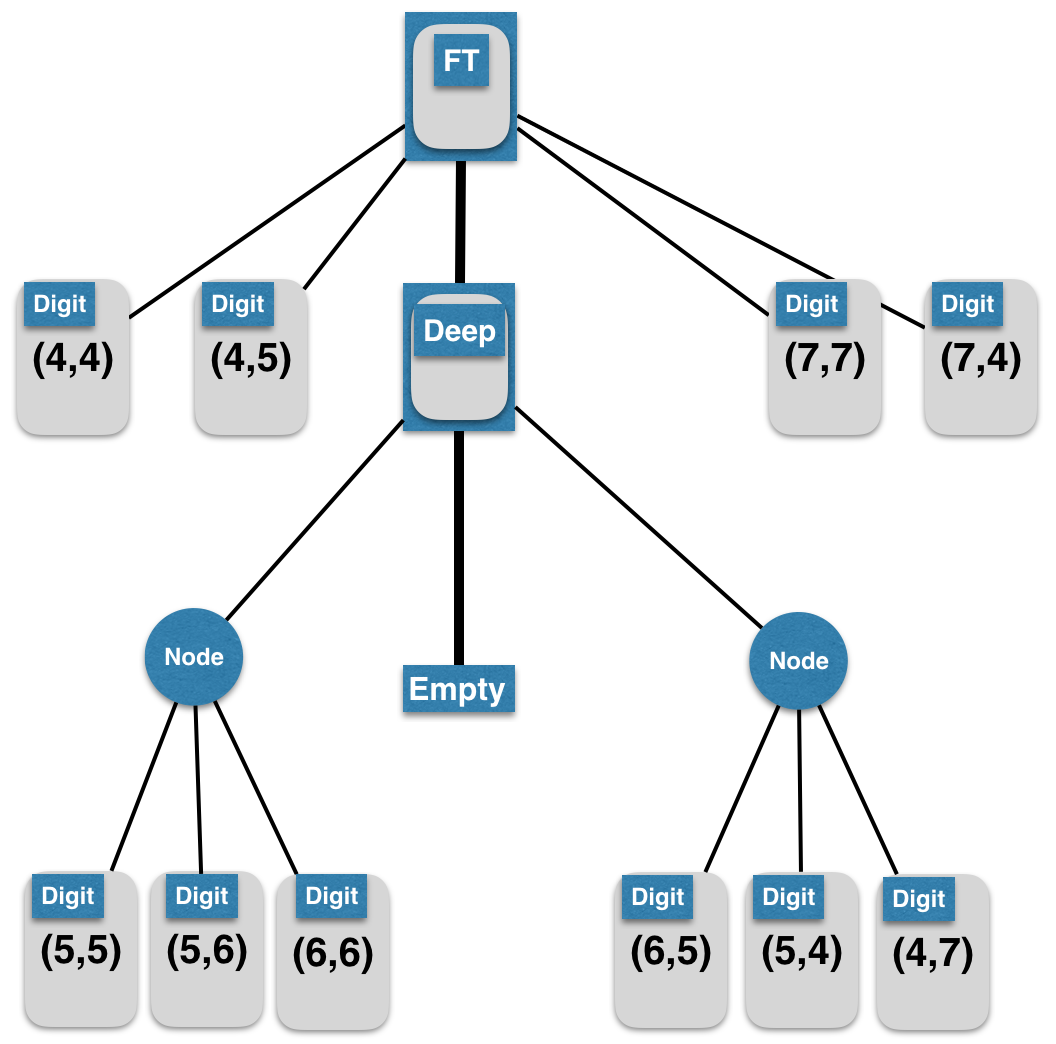
\includegraphics[scale=0.35]{./Images/FT-Euler-tour} 
\end{center}
\caption{A finger tree (FT) holding the sequence (Euler-tour) that represents the $k$-tree in Fig.\ref{fig:Euler-tour}}
\label{fig:FT-Euler-tour}
\end{figure}

Since the backbone of our structure \dyntset is actually a Hinze's and Paterson finger tree \cite{FTs}, we show the functions involved in our proposal, those to deal with inserting, cutting, appending and accessing finger trees. There are plenty of additional functions from finger trees we do not cover and that can be reached at \url{http://hackage.haskell.org/package/fingertree-0.1.4.1/docs/Data-FingerTree.html}.

\small
\begin{table}[H]
\begin{center}
\begin{tabular}{||l | l | c||} 
 \hline
 Function         & Type                                   & 
      \begin{tabular}{c} Time complexity \\ 
                         (amortised bounds)
      \end{tabular} \\
 \hline\hline
 \texttt{viewl}   & 
      \begin{tabular}{l} \texttt{FingerTree v a}   \\ 
                         \texttt{$\to$ ViewL (FingerTree v a)  } 
      \end{tabular}
                  & $\O(1)$ \\ 
 \hline
 \texttt{search}  & 
      \begin{tabular}{l} \texttt{(v $\to$ v $\to$ Bool)}   \\ 
                         \texttt{$\to$ FingerTree v a  }   \\ 
                         \texttt{$\to$ SearchResult v a  } 
      \end{tabular}
          & $\O(\log(min(i,n-i)))$  \\ 
 \hline
 \texttt{$\lhd$} (ins. from left) & 
      \begin{tabular}{l} \texttt{a $\to$ FingerTree v a} \\
                         \texttt{$\to$ FingerTree v a} 
      \end{tabular}
          & $\O(1)$                \\
 \hline
 \texttt{$\rhd$} (ins. from right) & 
      \begin{tabular}{l} \texttt{FingerTree v a $\to$ a} \\
                         \texttt{$\to$ FingerTree v a} 
      \end{tabular}
          & $\O(1)$                \\
 \hline
 \texttt{$\bowtie$} (concatenation) & 
      \begin{tabular}{l} \texttt{FingerTree v a} \\
                         \texttt{$\to$ FingerTree v a} \\
                         \texttt{$\to$ FingerTree v a} 
      \end{tabular}
          & $\O(\log ( min(m,n) ))$         \\
 \hline
\end{tabular}
\caption{Hinze's and Paterson implementation of \code{Data.FingerTree} \cite{FTsURL}, based on \cite{FTs}}
\label{tab:FTfuncs} 
\end{center}
\end{table}
\normalsize

where $n$ is the size of the largest sequence, $m$ is the size of the smaller sequence (i.e. when concatenating) and $i$ is the index of the element when searching. 

\tcb{SPLIT is not longer used, instead there is SEARCHFT, which aim is the same as SPLIT and hope it will be easier to explain}

\tcb{Is it the ``best" part in the document to bring up an explanations or examples or both for amortisation?}

%%%% END OF PRLIM
%%%% START OF EXAMPLE

\section{Example}
\label{sec:Example} 

In this section, we provide an example of the ETFT interface by depicting the core structure (i.e. finger tree) with internal vertices (i.e. sets) and sequences of pairs on the leaves (i.e. tours). Also, we illustrate the steps for computing \textit{split}s, \textit{insertion}s, \textit{concatenation}s, and lookups or \textit{view}s. All these the supporting functions to \textit{link} and \textit{cut} operations. Later, in Section~\ref{sec:TechDes}, we define these functions precisely describing their performance. 

\tcr{The whole section 3 is clumsy. Some of the pictures are useful to explain the idea of the annotations, but in many cases neither the text nor the figure add much information to what is already obviously from the name and type signature.}



Let us define two trees, $t_8$ and $t_2$. In this case we will consider the top vertex as the root, although, this is arbitrary and we can \textit{reroot} the tree at an existent vertex at any time.

Firstly, we have the tree $t_8$ on the left in in Figure~\ref{fig:t1et1ft1}, followed by its (only) Euler tour representation $et_8$ and its finger tree $ft_8$. At the top of $ft_8$ we have the monoidal representation of the set-union operation (shadowed ellipse) over all the leaf-vertices containing the pairs from $et_8$.
\begin{figure}
\begin{center}
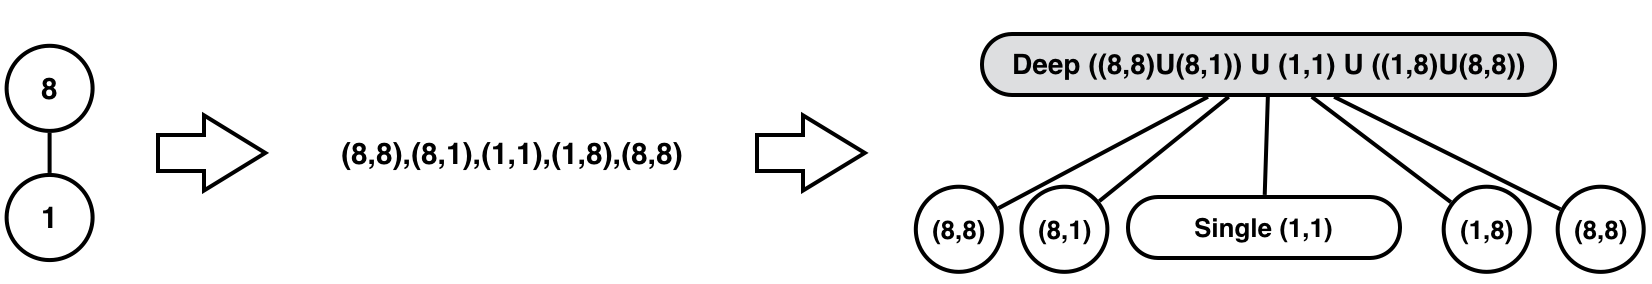
\includegraphics[scale=0.35]{./Images/t1et1ft1} 
\end{center}
\caption{Tree $t_8$ and its corresponding Euler tour $et_8$ and finger tree $ft_8$}
\label{fig:t1et1ft1}
\end{figure}

As an second example, we have $t_2$, Figure~\ref{fig:t2et2ft2}. The spine of the finger tree now contains a \code{Single} type constructor altogether with a \code{Node3}. Again, shadowed ellipses refer to the monoidal annotations \code{Set} where the set-insertion and set-union take place \textit{automatically}.
\begin{figure}
\begin{center}
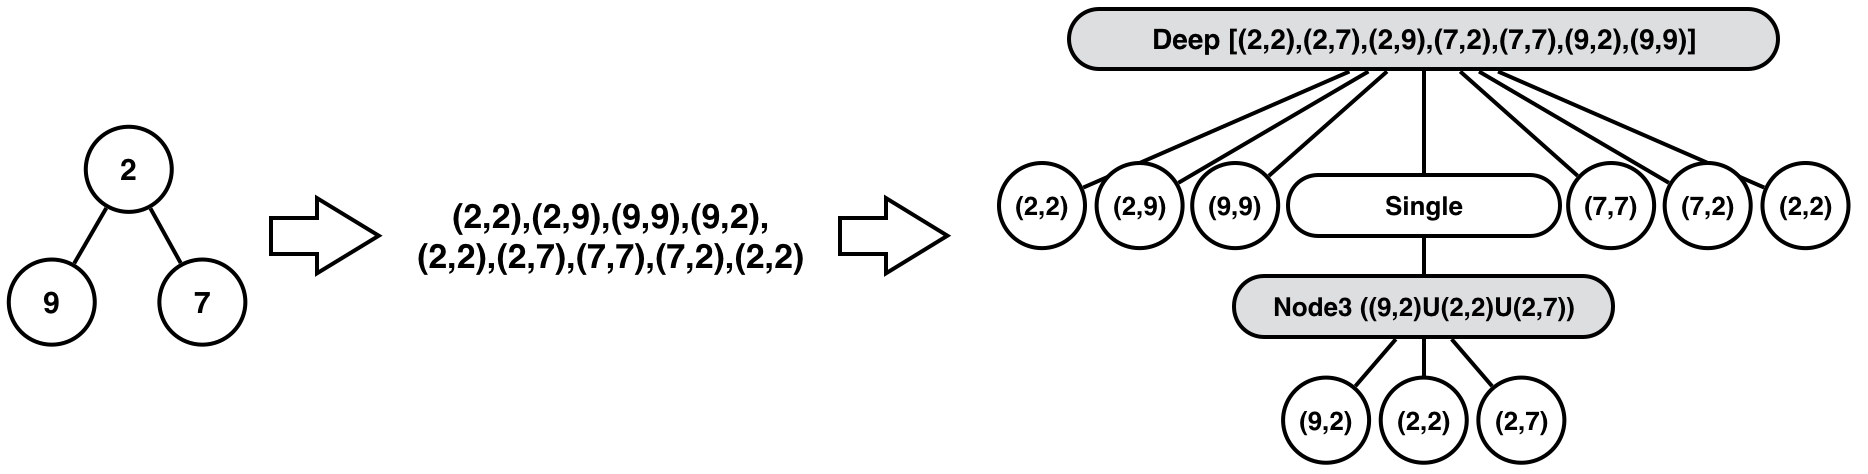
\includegraphics[scale=0.35]{./Images/t2et2ft2} 
\end{center}
\caption{Tree $t_2$ and its corresponding Euler tour $et_2$ and finger tree $ft_2$}
\label{fig:t2et2ft2}
\end{figure}

Now, the forest $f$ in Figure~\ref{fig:forest} is formed by inserting $ft_8$ and $ft_2$ from left and right respectively, in $\O(1)$. The forest's \code{Deep} type constructor has the set-union of all the finger trees ($ft_8$ and $ft_2$), depicted in back colour with white font. The thick lines coming out from the top ellipse are the components of the top finger tree: two \code{Digit} and an \code{Empty} subtree (or subforest).
\begin{figure}
\begin{center}
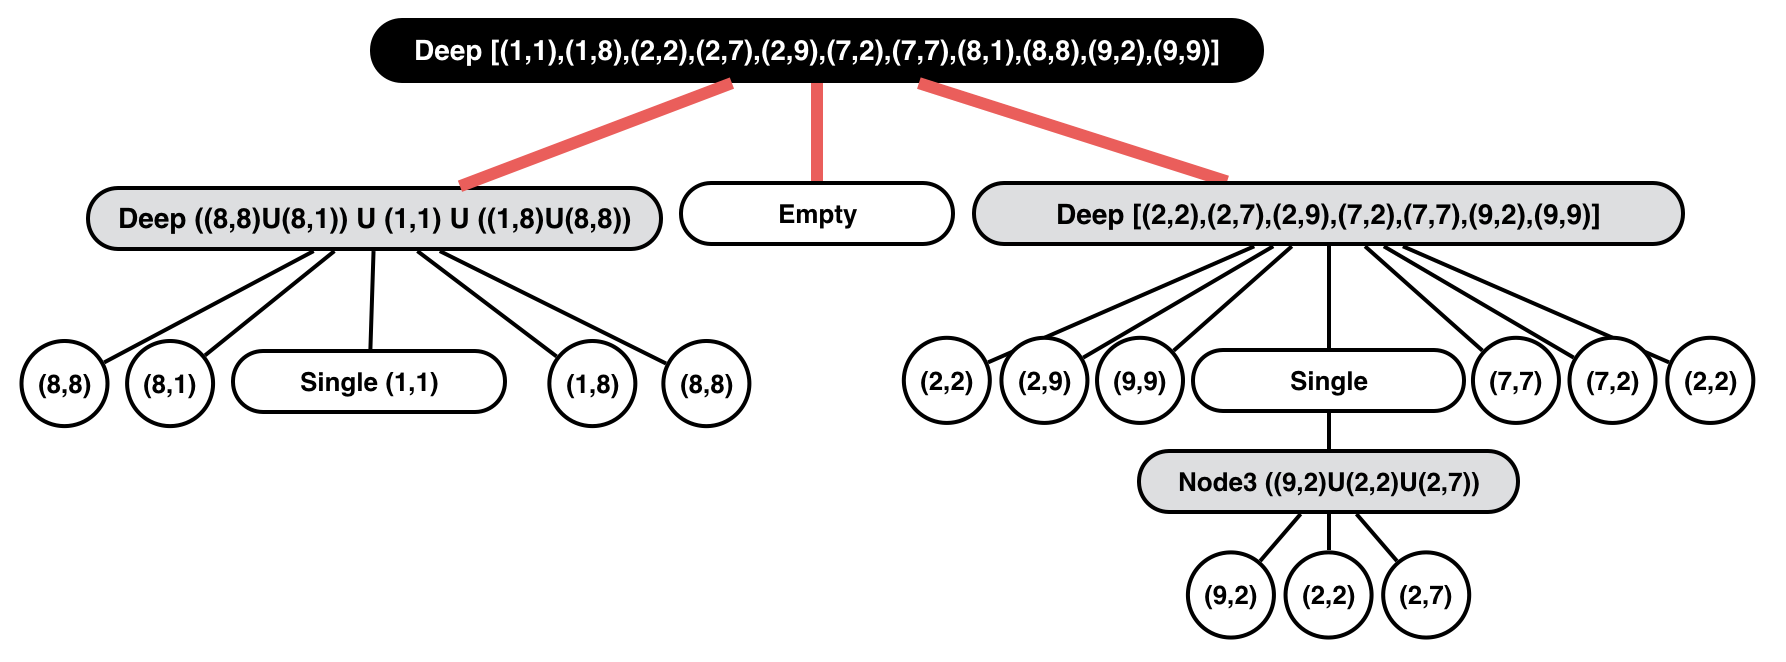
\includegraphics[scale=0.35]{./Images/forest} 
\end{center}
\caption{The forest $f$ comprising finger trees (Euler tours) as elements}
\label{fig:forest}
\end{figure}

Following, we have the basic operations for dynamic trees. Left side of Figure~\ref{fig:rootReroot} shows the \code{root} of a tree $t$ returning a vertex $v$, which is the first element of its finger tree $ft$, implemented in \code{viewl}. Rerooting a tree, by calling \code{reroot}, ask for a vertex $v$ and returns a \textit{new} tree. This is depicted in right side of Figure~\ref{fig:rootReroot}. This operation involves split, concatenation and insertions detailed in Section~\ref{sec:TechDes}.
\begin{figure}
\begin{center}
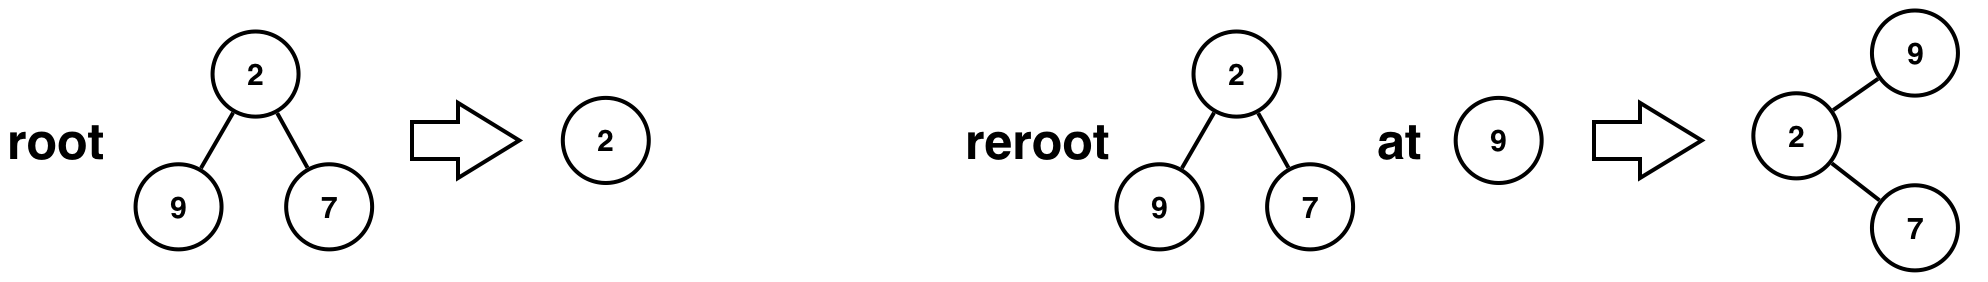
\includegraphics[scale=0.3]{./Images/rootReroot} 
\end{center}
\caption{\textit{root} and \textit{reroot} of a tree}
\label{fig:rootReroot}
\end{figure}

Splitting a finger tree, \code{split}, returns two subtrees (i.e. left and right) and an element, either a pair or an Euler tour, depending on the top container, a tree or a forest. This is depicted in Figure~\ref{fig:split}.
\begin{figure}
\begin{center}
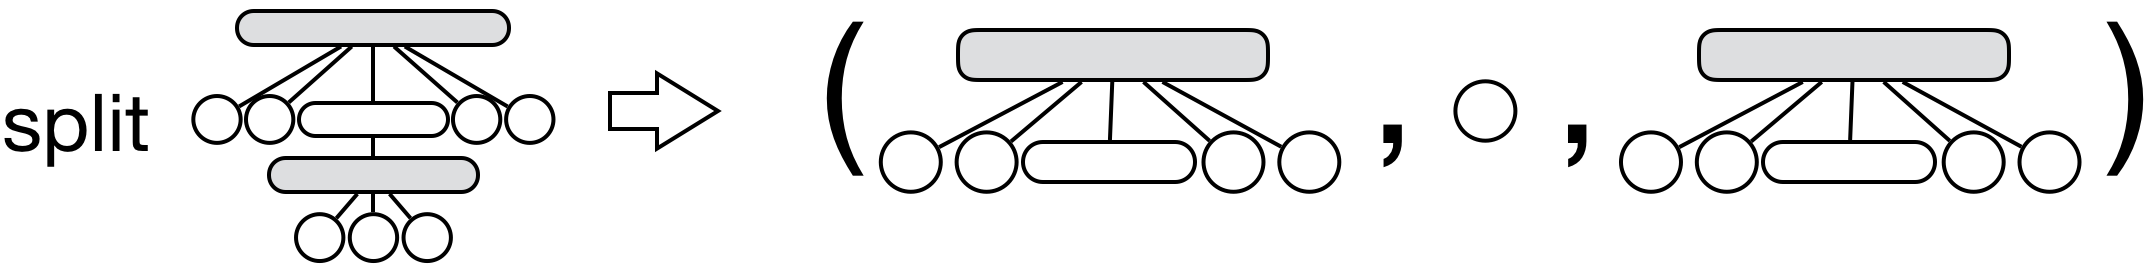
\includegraphics[scale=0.25]{./Images/split} 
\end{center}
\caption{Splitting a tree returns two smaller trees altogether an element}
\label{fig:split}
\end{figure}

Concatenating (also called appending) takes two finger trees and returns another (bigger) finger tree, as in Figure~\ref{fig:concatenation} and its represented by the $\bowtie$ symbol.
\begin{figure}
\begin{center}
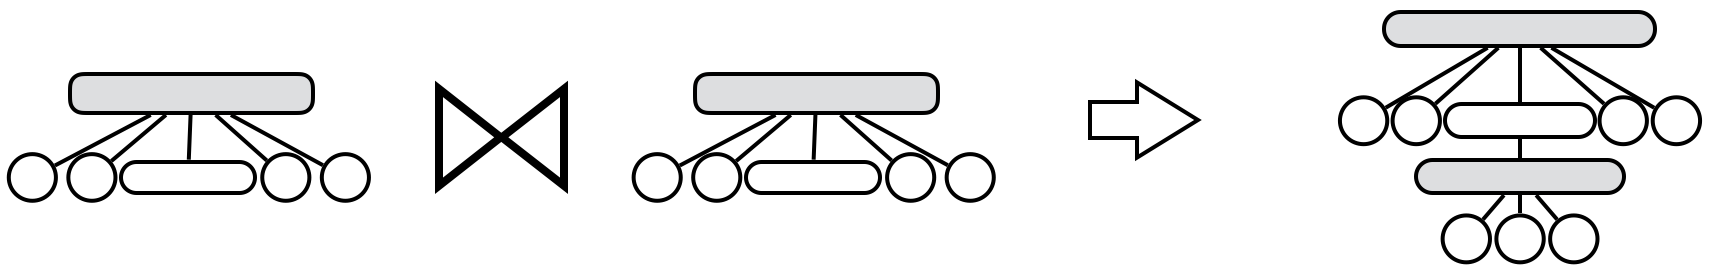
\includegraphics[scale=0.25]{./Images/concatenation} 
\end{center}
\caption{Concatenating two trees, returns a new one bigger}
\label{fig:concatenation}
\end{figure}


\tcr{Since the split operation over finger trees is central to the code, the paper would benefit from a more thorough explanation than the current incomplete type signatures (Concretely I'm missing an explanation of split's two first arguments).}


\tcr{The paper heavily builds on finger trees and tries to explain what they are and how they work, but omit aspects that are crucial to the understanding of the paper. In particular the `split` function is not explained, only listed in Table 2, but used in almost every listing later in the paper. The type listed for `split` mentions an unexplained type constructor `Split` and its type does not match the uses of `split`. The explanation around Fig. 5 does not help. What are the two first arguments to `split`?}




Under Figure~\ref{fig:consleftsnocright} we depict the final four help-functions that support \textit{link} and \textit{cut}: \code{viewl}, $\lhd$ (or \textit{cons}), $\rhd$ (or \textit{snoc}) and \textit{viewr}.
\begin{figure}
\begin{center}
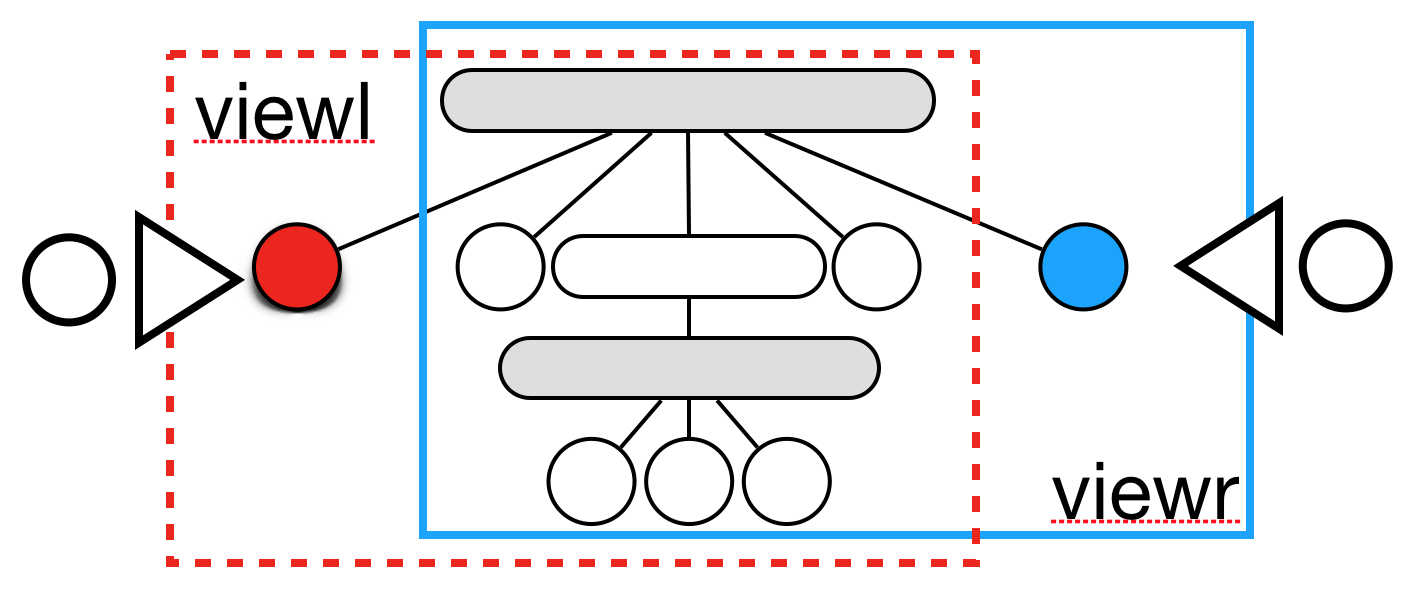
\includegraphics[scale=0.25]{./Images/consleftsnocright} 
\end{center}
\caption{Inserting and viewing from left (\code{viewl},$\lhd$) and inserting and viewing from right (\code{viewr},$\rhd$) }
\label{fig:consleftsnocright}
\end{figure}








%%%% END OF EXAMPLE
%%%% START OF TECHDES

\section{dynTsET Design}
\label{sec:TechDes}  

\tcr{My main criticism of the paper is the presentation. While I appreciate the use of diagrams in the first half of the paper, high-level explanations are missing later. The paper does not do a very good job providing an intuition for how the data structure works. For example, I was struggling understanding the role of the monoidal set. The paper also explains too little of the background regarding used existing data structures and their realisation in Haskell libraries. For example, the interface to the finger tree ADT and the Measured type class. In general, most of the explanations are closely tight to the code but don’t give a high-level picture of what individual operations do in terms of the Euler tour. Given that there is plenty of space left in the paper, this could be improved in the final version.}

\tcr{This reviewer can't help but think that there seems to be a lot of redundancy in the proposed data structure, as the Euler tour node pairs are present in both the sets and in the finger trees.}

In this section, we present the data types and the operations to manage dynamic trees through Euler-tour trees, that is \dyntset. Firstly, we describe how to convert any-degree tree into a Euler-tour tree. Secondly, assuming we are provided with Euler-tour trees, we define our initial data type which stores those trees within the leaves of a finger tree. Thirdly, we detail the functions for linking and cutting trees when performed in isolation. Finally, we incorporate the Euler-tour trees into the context of a forest. At this point, we describe the three operations regarded to dynamic trees: \conn (connectivity query), \link and \cut for trees within a forest. At any time, the number of nodes is fixed and every node is uniquely identified; nodes and edges are both represented as pairs. Full source code is located at \url{https://github.com/jcsaenzcarrasco/ETdynTs}.


\subsection{From $k$-degree tree to Euler-tour tree}

In Haskell, a $k-$degree tree (i.e. any-degree tree) is also known as multiway tree or rose tree. Actually, there is a library that defines such trees, \code{Data.Tree}, in the Haskell community's central package archive (Hackage).

\begin{lstlisting}
data Tree a = Node {
        rootLabel :: a,         
        subForest :: Forest a   
    }
\end{lstlisting}

So, a tree is a node of type \code{a} (i.e. its root) altogether with a list (possibly empty) of subtrees, seen as forest of type \code{Forest a}. Analogous to multiway trees, our trees (finger trees holding Euler-tours) can not be empty. 

Firstly, we turn a tree into a list of nodes, by attaching (mapping) the prefix and suffix of current node to inner subtrees. We later feed this list into a finger tree. The following function snippet can be read as \textit{rose-tree-to-euler-tour-tree}.

\begin{lstlisting}[mathescape] 
rt2et :: (Eq a) $\Rightarrow$ Tree a $\to$ [(a,a)] 
rt2et (Node x ts) = case ts of
  [] $\to$ [(x,x)]
  _  $\to$ root ++ concat ( map ($\lambda$t $\to$ pref t ++ rt2et t ++ suff t) ts )   
    where
     pref v = [(x,rootLabel v)]
     suff v = [(rootLabel v,x)]
     root   = [(x,x)] 
\end{lstlisting} 

Since \code{concat} and \texttt{++} take $\O(n)$ where $n$ is the size of the input tree, \code{rt2et} takes $\O(n)$. \tcr{Should we need to prove this ???}

The corresponding forest transformation to list of pairs is simply the application of \code{rt2et} to every element in the tree list. Because it requires a single traversal, \code{rf2et} (read as \textit{rose-forest-2-euler-tour-tree}) requires $\O(n)$ time, where $n$ is the number of elements in the forest. 

\begin{lstlisting}[mathescape] 
rf2et :: (Eq a) $\Rightarrow$ Forest a $\to$ [[(a,a)]]
rf2et []          = []
rf2et [Node x []] = [[(x,x)]]  
rf2et (t:ts)      = (rt2et t) : rf2et ts
\end{lstlisting}

Once a tree $t$ of any degree is turned into an Euler tour $et$, we are able to manage $et$ as a sequence. 


\subsection{Euler-tour tree as finger tree of pairs with a set of pairs as monoidal annotation}

Since finger trees work efficiently on sequences, according to \cite{FTs} (see also Table~\ref{tab:FTfuncs}), we tailored the finger tree in order to support \link, \cut and \conn operations over unrooted trees following the procedures for modifying encodings (i.e. conversions between any-degree tree and Euler-tours) by Henzinger and King in \cite{Rand-DynGs-Algos}.

Recall from Figure~\ref{fig:FTdatatype}, the finger tree \code{data FingerTree v a}, has two polymorphic types, the first one (\code{v}) is the type of the monoidal annotation and the second (\code{a}) the type of the values stored at the leaves, which in our case is the sequence type. In Section~\ref{sec:ETt} we provided the need for nodes and edges to be treated as pairs (see also Figure~\ref{fig:Euler-tour}), therefore our values type is \code{(a,a)} for any type \code{a}, although in the following sections we will define such pairs as integers for practical purposes. In this manner, a pair $(u,v)$ (atomic element in the sequence) represents a node, when $u = v$, and an edge when $u \neq v$. From here, every element in the sequence can be located.

For the internal finger tree nodes (monoidal annotations), where searching take place, we define \code{Data.Set (a,a)} as our type. By doing so, we are able to take advantage from some set-like operations such as membership-test, insertion and union. 

We define the set-insertion operation every time a pair (either edge or node) is added to an Euler-tour tree (i.e. finger tree). The set-union is already defined in \code{Data.Set} at its monoidal binary operation, therefore there is no need to define this in our proposal. Testing membership is performed through the finger tree \code{search} function \cite{FTsURL}. Our data type for holding a sequence (Euler-tour tree) whithin a finger tree is called \code{TreeEF} defined below followed by its corresponding instance for \textit{measuring} it, that is, returning a set when a value is provided.

\begin{lstlisting}[mathescape]
import qualified Data.FingerTree as FT
import qualified Data.Set        as S

type TreeEF   a = FingerTree (S.Set (a,a)) (a,a)

instance (Ord a) $\Rightarrow$ Measured (S.Set (a,a)) (a,a) where 
   measure (x,y) = S.insert (x,y) S.empty 
\end{lstlisting} 

In the context of performance, we recall finger tree functions (see Table~\ref{tab:FTfuncs}). At that stage, every function assumes the monoidal annotation takes $\O(1)$. Since our annotation is not a simple type, we calculate the corresponding finger tree operations into our \dyntset proposal as:
\begin{itemize}
\item \code{viewl}: remains the same as there is no further operations involved, that is, $\O(1)$.
\item $\lhd$: since the insertion takes place through a set-insertion, then we have $\O(\log n)$ replacing $\O(1)$.
\item $\rhd$: same as $\lhd$
\item $\bowtie$: concatenation involves the set-union operation at the monoidal annotation nodes. Then, let $m$ and $n$ be the sizes of the sets every time there is a union operation performed. Following the performance and constraint from Table~\ref{tab:Setfuncs}, we have $\O(m(\log\frac{n}{m} +1))$. If $m$ is 1, that is, inserting a single element in a set of size $n$ (as in $\lhd$ or $\rhd$) we have $\O(1(\log\frac{n}{1} +1))$ which turns $\O(\log n)$. If $m$ is at most $n$, then $\O(n(\log\frac{n}{n} +1))$, resulting in $\O(n)$. Although the latter case (the worst) might be presented at any time, it is not always the case when concatenating since sizes of the sets in a finger tree are not constant, either growing up to $n$ for both sets or shrinking down to 1 for one set. In any case, for $\bowtie$ we have $\O(\log(min(m,n)))$ where $m$ and $n$ might get $n^2$, hence $\O(\log n^2)$.
\item \code{search}: every search in the finger tree uses a test-membership in the monoidal annotations nodes which takes $\O(\log n)$. Then, the $\O(\log(min(i,n-i)))$ is substituted by $\O(\log (\log n))$, resulting in $\O(\log^2 n)$. Although this just the calculation of the performances of a set within a finger tree. Since a finger tree (non singular) has a monoidal annotation on its top (line 3 in Figure~\ref{fig:FTdatatype}) the look up for an element is actually a simple test-membership operation, that is, $\O(\log n)$. 
\end{itemize}

Summarising the above, the following are the types and bounds for \dyntset, provided type \code{v} is actually \code{Set b} and type \code{b} is actually the pair \code{(a,a)}

\small
\begin{table}[H]
\begin{center}
\begin{tabular}{||l | l | c||} 
 \hline
 Function         & Type                                   & 
      \begin{tabular}{c} Time complexity \\ 
                         (amortised bounds)
      \end{tabular} \\
 \hline\hline
 \texttt{viewl}   & 
      \begin{tabular}{l} \texttt{FingerTree v b}   \\ 
                         \texttt{$\to$ ViewL (FingerTree v b)  } 
      \end{tabular}
                  & $\O(1)$ \\ 
 \hline
 \texttt{search}  & 
      \begin{tabular}{l} \texttt{(v $\to$ v $\to$ Bool)}   \\ 
                         \texttt{$\to$ FingerTree v b  }   \\ 
                         \texttt{$\to$ SearchResult v b  } 
      \end{tabular}
          & $\O(\log n)$  \\ 
 \hline
 \texttt{$\lhd$}  & 
      \begin{tabular}{l} \texttt{b $\to$ FingerTree v b} \\
                         \texttt{$\to$ FingerTree v b} 
      \end{tabular}
          & $\O(\log n)$                \\
 \hline
 \texttt{$\rhd$}  & 
      \begin{tabular}{l} \texttt{FingerTree v b $\to$ b} \\
                         \texttt{$\to$ FingerTree v b} 
      \end{tabular}
          & $\O(\log n)$                \\
 \hline
 \texttt{$\bowtie$}  & 
      \begin{tabular}{l} \texttt{FingerTree v b} \\
                         \texttt{$\to$ FingerTree v b} \\
                         \texttt{$\to$ FingerTree v b} 
      \end{tabular}
          & $\O(\log n^2)$         \\
 \hline
\end{tabular}
\caption{\dyntset types and performances}
\label{tab:dyntsetFTfuncs} 
\end{center}
\end{table}
\normalsize

\subsection{rooting and rerooting a tree}
Functions \root and \reroot play a crucial importance in the definition of \link, \cut and \conn as we shall see shortly. We mentioned earlier that dynamic trees is about managing unrooted trees. By \root we refer to the entry point of any Euler-tour, which always starts in the form $(v,v)$ since it represents a node. By \emph{unrooted} tree we refer to the fact that any node in the tree can be its \root. This is actually performed in function \link.

We have showed that \code{viewl} returns the leftist element of a finger tree. Applying \code{viewl} a \code{TreeEF} we have its root as in the following snippet.
\begin{lstlisting}[mathescape] 
root :: Ord a $\Rightarrow$ TreeEF a $\to$ Maybe a  
root tree = case viewl tree of
  EmptyL   $\to$ Nothing
  x :< _   $\to$ Just ( fst x )
\end{lstlisting}

We return the first element in the pair $(v,v)$ since any $v$ represents the node-root. Time complexity of \root is $\O(1)$ since \code{viewl} performs $\O(1)$ in the finger tree and we simply pattern match over its results.

Then, for \textit{reroot}ing a tree we follow the second procedure by Henzinger and King in \cite{Rand-DynGs-Algos}, which states:
\begin{displayquote}
\emph{To change the root of \textit{T} from $r$ to $s$}: Let $o_s$ denote any occurrence of $s$. Splice out the first part of the sequence ending with the occurrence before $o_s$, remove its first occurrence ($o_r$), and tack the first part on to the end of the sequence, which now begins with $o_s$. Add a new occurrence $o_s$ to the end.
\end{displayquote}

So, instead of looking for $r$ (old root) occurrences, we focus only in the new root($s$). We splice out the first and second occurrences of node $s$ by simply searching for it as $(s,s)$ in the finger tree: \code{S.member (s,s) tree}. Then, simply glue all the parts in order, that is, the new root first (leftist) followed by the second and first occurrences of $s$: \code{(s,s)} $\lhd$ \code{(right } $\bowtie$ \code{ left)}. This is denoted in the following snippet.

\begin{lstlisting}[mathescape] 
reroot :: Ord a $\Rightarrow$ TreeEF a $\to$ a $\to$ TreeEF a 
reroot tree node = case (FT.search pred tree) of
   Position left _ right $\to$ rootTree $\lhd$ (right $\bowtie$ left)
   _                     $\to$ tree
 where rootTree      = (node,node)
       pred before _ = (S.member rootTree) before
\end{lstlisting} 

\tcr{PERFORMANCE of REROOT }\tcb{Operators $\lhd$, \code{FT.search}, and $\bowtie$ take $\O(1)$, $\O(\log n)$ and $\O(\log n^2)$ amortised respectively on finger trees. Since we are applying them only once, our \reroot function also takes $\O(\log n^2)$}. In case \reroot is asked altogether with a node not in the tree, it simply returns the original \code{tree} (fourth line in above snippet).


\subsection{linking and cutting trees off the forest}

For cutting a tree or deleting an edge following Henzinger and King in their first procedure in \cite{Rand-DynGs-Algos} we have:
\begin{displayquote}
\emph{To delete edge \{$a$,$b$\} from $T$:} Let $T_1$ and $T_2$ be the two trees that result, where $a \in$ $T_1$ and $b \in$ $T_2$. Let $o_{a_1}$, $o_{b_1}$, $o_{b_2}$ represent the occurrences encountered in the two traversals of \{$a,b$\}. If $o_{a_1} < o_{b_1}$ and $o_{b_1} < o_{b_2}$, then $o_{a_1} < o_{b_1} < o_{b_2} < o_{a_2}$. Thus, ET($T_2$) is given by the interval of ET($T$) $o_{b_1}$, \ldots, $o_{b_2}$ and ET($T_1$) is given by splicing out of ET($T$) the sequence $o_{b_1}$, \ldots, $o_{a_2}$. 
\end{displayquote} 

The following snippet shows the \code{cutTree} operation analogous to the above procedure :
\begin{lstlisting}[mathescape]
cutTree :: Ord a $\Rightarrow$ a $\to$ a $\to$ TreeEF a $\to$ Maybe (TreeEF a,TreeEF a) 
cutTree u v tree = case FT.search predUV tree of
 Position left _ right $\to$
   case (FT.search predVU left ) of
      Position leftL _ rightL $\to$  
        Just (rightL, leftL $\bowtie$ right)
      _                $\to$                    
        case (FT.search predVU right) of
          Position leftR _ rightR $\to$
            Just (leftR, left $\bowtie$ rightR)
          _ $\to$ Nothing 
 _  $\to$ Nothing  
 where
   predUV before _ = (S.member (u,v)) before 
   predVU before _ = (S.member (v,u)) before 
\end{lstlisting}

The snippet quite follows the procedure. The pairs $(u,v)$ and $(v,u)$ are left out the resulting sequences in the wildcards in lines 3, 5 and 9. Since we search $(u,v)$ first, there are only two possibilities for $(v,u)$ to be part of. If it is on the left we build up $T_1$ from \code{rightL}, and $T_2$ from \code{leftL} and \code{right}. Otherwise $T_1$ is built from \code{leftR} and $T_2$ from \code{left} and \code{rightR}. $T_2$ is spliced out through the $\bowtie$ operator.

\tcr{PERFORMANCE of cutTree }\tcb{Operator $\bowtie$ and function \code{FT.search} take $\O(\log n^2)$ and $\O(\log n)$ amortised respectively on finger trees. Since we are applying $\bowtie$ once and \code{search} twice, then \code{cutTree} function also takes $\O(\log n^2)$}. In case \code{cutTree} is called with nodes belonging different components (edge not in \code{tree}), then \code{cutTree} returns \code{Nothing} in $\O(\log n)$, which will be captured as failure in \cut within a forest operation.


Now, for linking a tree (or joining two trees), we follow the third and final encoding in \cite{Rand-DynGs-Algos}:
\begin{displayquote}
\emph{To join two rooted trees $T$ and $T'$ by edge $e$:} Let $e = \{a,b\}$ with $a \in T$ and $b \in T'$. Given any  occurrence $o_a$ and $o_b$, reroot $T'$ at $b$, create a new occurrence $o_{a_n}$ and splice the sequence $ET(T')o_{a_n}$ into $ET(T)$ immediately after $o_a$.
\end{displayquote} 

The following snippet translate the above procedure quite close. 
\begin{lstlisting}[mathescape]
linkTree :: Ord a $\Rightarrow$ a $\to$ TreeEF a $\to$ a $\to$ TreeEF a $\to$ Maybe (TreeEF a) 
linkTree u tu v tv = case (pairIn (u,u) tu, pairIn (v,v) tv) of
  (False, _    ) $\to$ Nothing
  (_    , False) $\to$ Nothing 
  (True , True ) $\to$ Just $\$$
    let from = reroot tu u
        (Position left _ right) = FT.search pred tv
    in  ((left $\rhd$ (v,v)) $\rhd$ (v,u)) $\bowtie$ from $\bowtie$ ((u,v) $\lhd$ right)
 where
   pred before _ = (S.member (v,v)) before
\end{lstlisting} 

We build $e = \{a,b\}$ where $a \in T$ and $b \in T'$ from the procedure in line 2 as \code{(u,u)} $\in$ \code{tu} and \code{(v,v)} $\in$ \code{tv}.  Then, in line 6, we reroot $T'$ at $b$ as \code{reroot tu u} calling its result as \code{from} and finally splicing it in line 8 immediately after \code{(v,u)}. 

\tcr{PERFORMANCE of linkTree.} We have two times the performance of \code{search} within \code{pairIn} (line 2 above), that is, $\O(\log n)$. Then we call \code{search} one more time at line 7. Finally we build up the resulting tree by applying $\lhd$ and $\rhd$ taking $\O(1)$ and $\bowtie$ taking $\O(\log n^2)$ time. Function \code{pairIn} is defined as 
\begin{lstlisting} [mathescape]
pairIn :: (Measured (S.Set a) a, Ord a)
       $\Rightarrow$ a $\to$ FingerTree (S.Set a) a
       $\to$ Bool
pairIn p monFT = case (FT.search pred monFT) of
  Position _ _ _ $\to$ True 
  _              $\to$ False
 where
   pred before _ = (S.member p) before 
\end{lstlisting} 


\subsection{\link, \cut and \conn within a forest} 
Literature refers to link and cut operations (as in \cite{DS-DynTs}, \cite{WerneckR-PhD} and \cite{Rand-DynGs-Algos}) to the definitions and analysis we have done previously. In this part, we shall see that \link, \cut specialise the former ones in the context of a forest. Moreover, \conn answers the queries for \textit{connectivity} in the dynamic setting, that is, given an finite sequence of link and cut operations applied to a forest, \conn returns \code{True} if the two nodes provided belong to the same component (tree) within a forest, or \code{False} otherwise. 

Firstly, we need to define a data type for a forest structure. In Section~\ref{sec:Prelim} we defined a tree as Euler-tour, which is now the leaf in the forest-finger-tree structure i.e. its \textit{element}. Likewise the internal nodes in a tree, a set is also the monoidal annotation in the forest type. The result, a finger tree comprised of finger trees.
\begin{lstlisting}[mathescape] 
type ForestEF a = FingerTree (S.Set (a,a)) (TreeEF a) 
\end{lstlisting} 

The fastest and easiest operation is \conn. It simply tests membership for each node against the top set in the forest, that is, the monoidal annotation in the root of the finger tree: \code{nodeIn node forest}. Then, if both nodes are elements of the forest implies they belong to a tree, remaining the question for whether or not both roots are the same
\begin{lstlisting}[mathescape]
conn :: Ord a $\Rightarrow$ a $\to$ a $\to$ ForestEF a $\to$ Bool
conn x y f =
 case (nodeIn x f, nodeIn y f) of 
  (Just (tx,rx) , Just (ty,ry)) $\to$ if rx == ry  then True else False
  _                             $\to$ False
\end{lstlisting}

Notice we have not searched pairs of nodes but the nodes themselves. This is evaluated internally in \code{nodeIn} function.
\begin{lstlisting}[mathescape]
nodeIn :: Ord a $\Rightarrow$ a $\to$ ForestEF a $\to$ Maybe (TreeEF a, a) 
nodeIn node forest = 
 case FT.search pred forest of 
  Position _ tree _ $\to$
     case (root tree) of
       Nothing    $\to$ Nothing 
       Just rootT $\to$ Just (tree, rootT) 
  _                 $\to$ Nothing    
 where
   pred before _ = (S.member (node,node)) before 
\end{lstlisting} 

Following the bounds from Table~\ref{tab:dyntsetFTfuncs} we have that \code{nodeIn}, called only twice, applies \code{root} which takes $\O(1)$ and \code{FT.search} which takes $\O(\log n)$, thus querying for connectivity in our structure through \conn takes $\O(\log n)$. 

Similar to \code{cutTree}, \cut requires two nodes as arguments, but alike \code{cutTree} requires:
\begin{itemize}
\item [req$_{c1}$]: a forest instead of a tree, although the tree is searched rather than provided;
\item [req$_{c2}$]: the tree where the nodes belong to is left out of the forest;
\item [req$_{c3}$]: the resulting trees from cutting are inserted into the \textit{new} forest (from the left)
\end{itemize}

By {\cut}ting trees the forest increases its number of trees, from two when the forest has a single tree up to the number of nodes when each tree does not have children.

\begin{lstlisting}[mathescape] 
cut :: Ord a $\Rightarrow$ a $\to$ a $\to$ ForestEF a $\to$ ForestEF a 
cut x y forest  
 | x == y    = forest  
 | otherwise = 
    case connected x y forest of 
      (True, Just (tx,_,_,_)) $\to$ case (cutTree x y tx) of
        Nothing     $\to$ forest 
        Just result $\to$ buildForest result  
      _                       $\to$ forest 
 where 
    buildForest (t2,t3) = t2 $\lhd$ (t3 $\lhd$ (lf $\bowtie$ rf)) 
    Position lf _ rf    = FT.search pred forest
    pred before _       = (S.member (x,x)) before
\end{lstlisting} 

In \dyntset, \cut does not assume nodes belong to the tree. We verify this in lines 5 and 6. req$_{c1}$ is discharged in line 6 i.e. \code{tx}; req$_{c2}$ is fulfilled in line 12 through the wildcard \code{_}. req$_{c3}$ is met through \code{buildForest} function in line 11. 

\tcr{PERFORMANCE of \cut }\tcb{We perform $\O(\log n)$ in \code{connected} (line 5) as we shall see shortly. Later, \code{cutTree} in line 6 takes $\O(\log m^2)$. Here, $n$ represents the number of nodes in the forest and $m$ the number of nodes in \code{tx} (i.e. local tree). In case the forest is comprised of a single tree i.e. $m = n$, then \code{cutTree} takes $\O(\log n^2)$. Function \code{buildForest}, defined at line 11, takes $2T_1(\lhd)+T_2(\bowtie)$. The function $T_1$ is the time taken for gluing (inserting) the resulting trees from cutting, \code{t2} and \code{t3}, into the forest. Function $T_2$ is the time taken of gluing (concatenating) the subforest \code{lf} and subforest \code{rf}. This concatenation is the effect of leaving apart the cut tree, \code{tx}. Since both $T_1$ and $T_2$ operate over the forest, $n$ is the variable. Then, $T_1 = \O(\log n)$ and $T_2 = \O(\log n^2)$ following the performance from Table~\ref{tab:dyntsetFTfuncs}. Thus, \cut takes up to $\O(\log n^2)$ amortised time. }

We take advantage from function \code{nodeIn} to define \code{connected} as auxiliary function for \cut and \link. Here is its definition.
\begin{lstlisting}[mathescape] 
connected :: Ord a $\Rightarrow$ a $\to$ a $\to$ ForestEF a
          $\to$ (Bool, Maybe (TreeEF a, a, TreeEF a, a) ) 
connected x y f = 
 case (nodeIn x f, nodeIn y f) of 
  (Just (tx,rx)     , Just (ty,ry)) $\to$ if rx == ry 
                                   then (True,  Just(tx,rx,tx,rx))  
                                   else (False, Just(tx,rx,ty,ry)) 
  _                                 $\to$ (False, Nothing) 
\end{lstlisting} 
Function \code{connected} takes twice the time as \code{nodeIn} as this is called once per node. The remaining code is just pattern matching. 

The \link operation follows the same pattern than \cut operation. The difference is the application of \code{linkTree} and the construction of the \textit{new} forest. Also, similar to \cut, \link requires:
\begin{itemize}
\item [req$_{l1}$]: a forest instead of a tree, although the tree is searched rather than provided, satisfied through \code{connected} as in \cut.
\item [req$_{l2}$]: the trees where the nodes belong to are left out of the forest, two steps rather than one as in \cut
\item [req$_{l3}$]: the resulting tree from linking is inserted into the \textit{new} forest (from the left)
\end{itemize}

\begin{lstlisting}[mathescape] 
link :: Ord a $\Rightarrow$ a $\to$ a $\to$ ForestEF a $\to$ ForestEF a 
link x y forest 
  | x == y    = forest  
  | otherwise = 
     case connected x y forest of 
      (False, Just (tx,rx,ty,ry)) $\to$ case (linkTree x tx y ty) of
         Nothing     $\to$ forest
         Just result $\to$ linkAll result 
      _                           $\to$ forest 
 where 
    Position lf' _ rf' = FT.search predX forest 
    Position lf  _ rf  = FT.search predY (lf' $\bowtie$ rf') 
    linkAll tree    = tree $\lhd$ (lf $\bowtie$ rf)
    predX before _ = (S.member (x,x)) before 
    predY before _ = (S.member (y,y)) before 
\end{lstlisting}
\tcr{PERFORMANCE of \link }. Following the bottom-up approach from the above snippet and the performances from Table~\ref{tab:dyntsetFTfuncs}, we have in line 11, the subforests \code{lf'} and \code{rf'} which get rid of the original tree containing node \code{x}. Then, in line 12, \code{lf} and \code{rf} are the subforests after disposing the original tree containing node \code{y} (wildcards \code{_} respectively). These two steps satisfy req$_{l2}$ and take twice the time of \code{FT.search} which is $\O(\log n)$ and once the time of $\bowtie$ at forest level which is $\O(\log n^2)$. Then \code{linkAll}, defined at line 13, calls $\lhd$ for inserting the \textit{new} \code{tree}, as \code{result} of \code{linkTree}, into the \textit{new} forest, taking $\O(\log n)$ altogether with the concatenation of \code{lf} and \code{rf} in $\O(\log n^2)$. With this, we meet req$_{l3}$. In line 5, we ensure to look for the nodes \code{x} and \code{y} within the \code{forest} in $\O(\log n)$. If both nodes are members of the \code{forest} but not connected, line 6, then \code{linkTree} is performed in $\O(\log m^2)$ where $m$ is the size of the sum of the number of the nodes in trees \code{tx} and \code{ty}, unless $\vert$\code{tx}$\vert + \vert$\code{ty}$\vert = n$, where \code{linkTree} takes $\O(\log n^2)$. Since no loop or recursion is involved and that of a constant number of operations were made in \link, this function takes up to $\O(\log n^2)$ amortised.






%%%% END OF TECHDES
%%%% START OF EVAL

\section{Experimental Evaluation} 
\label{sec:Eval} 


This section presents experiments to evaluate how much running time costs in terms of performance. The experiments will show that, in practice, \dyntset is faster by a factor of $\O(\log n)$ per operation than that of the theoretical analysis (Section\ref{sec:TechDes}).

This section is organised as follows. Firstly, we describe the experimental setup. Secondly, a brief description in the implementation of test sets is provided. We then present experimental studies of the three different operations in \dyntset. Finally, we present an additional experiment for the cases where laziness as speeding up factor in favor of the running times for the dynamic tree operations.


\subsection{Experimental Setup}
Functions \link, \cut, \conn, \code{root} and \code{reroot} were implemented by the author in Haskell and compiled with \code{ghc} version 8.0.1 with optimisation \code{-O2}. The experiments were performed on a 2.2 GHz Intel Core i7 MacBook Pro with 16 GB 1600 MHz DDR3 running macOS High Sierra version 10.13.1 (17B1003). We imported the following libraries into our code from the online package repository Hackage: \cite{HaskellFT} code for finger trees, \cite{HaskellSet} for conventional sets and \cite{HaskellEdison} for lazy sets.

The running time of a given computation was determined by the mean of three executions.

\subsection{Data structure} 

The values maintained by the data structures (sets and finger trees) are stored as fixed-precision \code{Int} types, holding values from $-2^{29}$ up to $2^{28}$ although we test only the positive values.

The structures are initialized with a fixed number of nodes (or vertices) $n$; this number does not change during the execution. This allow us to know the initial size of the forest and we subtract it from the benchmarking.

Since \dyntset is not called by any application, the random generation of nodes for \link or \cut does not necessarily be effective. Actually, around 70\% of the generated nodes $x$ and $y$ passed to \link and \cut were not valid, that is, their result turned out to be the original forest. In order to overcome this, we stored the random generated nodes that were effective into a plain files and from there benchmarking the dynamic tree operations.


\subsection{Incremental operations} 
We start with an empty forest (just singleton-trees); given $n=20,000$ nodes we perform $1 \ldots 20,000$ \link operations. Upon reaching a target length, we plot the total time taken. Then, we divide the time taken by the number of operations to calculate the time per operation and then multiply it by a constant (x1000) to make the curve visible in the same chart.

\begin{figure}[H]
\begin{center}
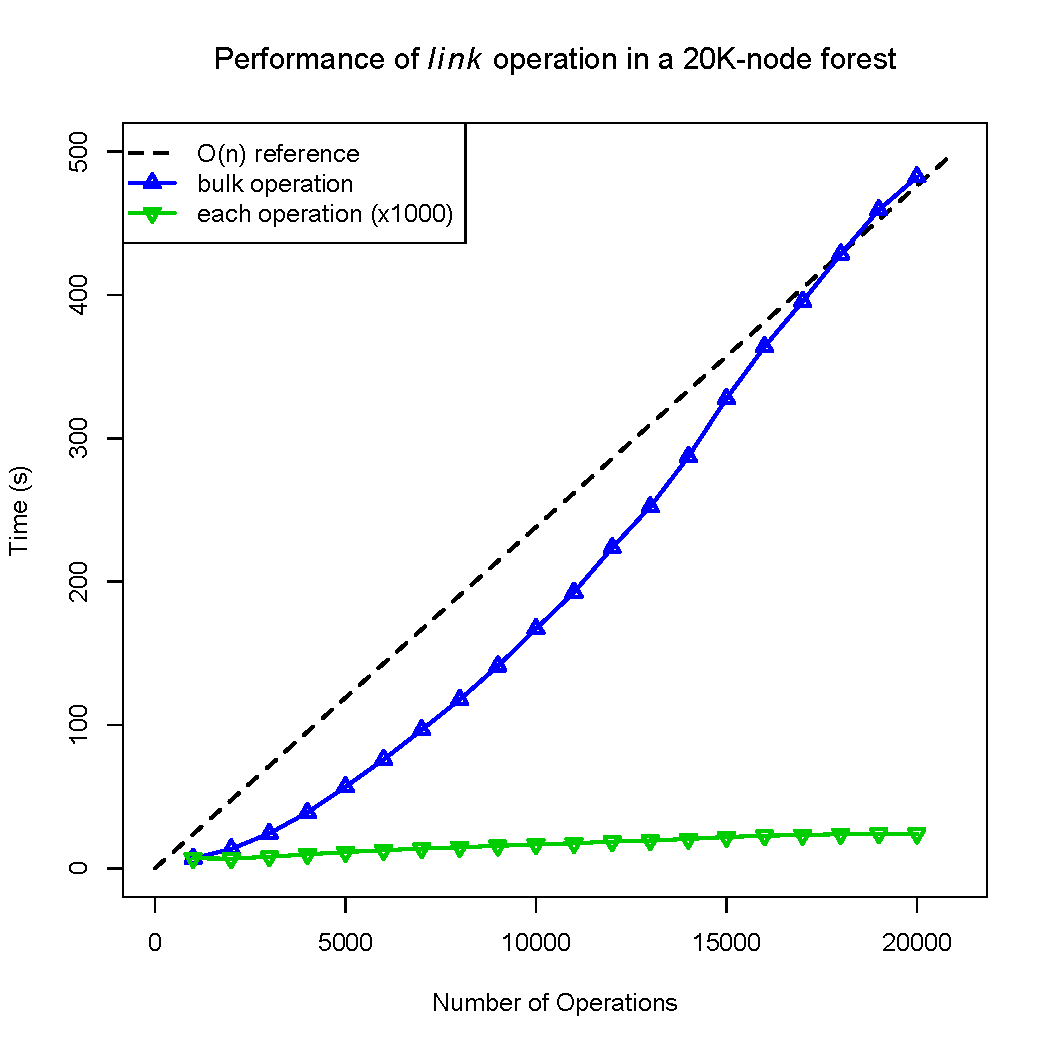
\includegraphics[scale=0.4]{./Images/plotLink} 
\end{center}
\caption{Sequence of {\link}s from empty forest up to a single tree in such forest}
\label{fig:incLink}
\end{figure}

\textit{\emph{Results}}. The behaviour of the curve regarding the time per \link operation shows that in practice it takes $\O(1)$ against $\O(\log n^2)$ in theory back in Section~\ref{sec:TechDes}, or the linear behaviour by the \link operations in bulk.

\subsection{Fully dynamic operations} 
We start with the incremental process as before for $n=10,000$. Then, for \cut we start in the opposite direction, that is, cutting from a single tree in the forest until only singleton-trees remain in such forest. To this performance we subtract the time take for the incremental bit. For \conn performance we compute first an interleaved operation of \link and \cut (not necessarily in this order). We measure the time taken for \conn followed by the corresponding \link or \cut and then we subtract the interleaved process. The following figures show our three dynamic operations in bulk and per operation.

\begin{figure}[H]
\centering
\begin{subfigure}{.5\textwidth}
  \centering
  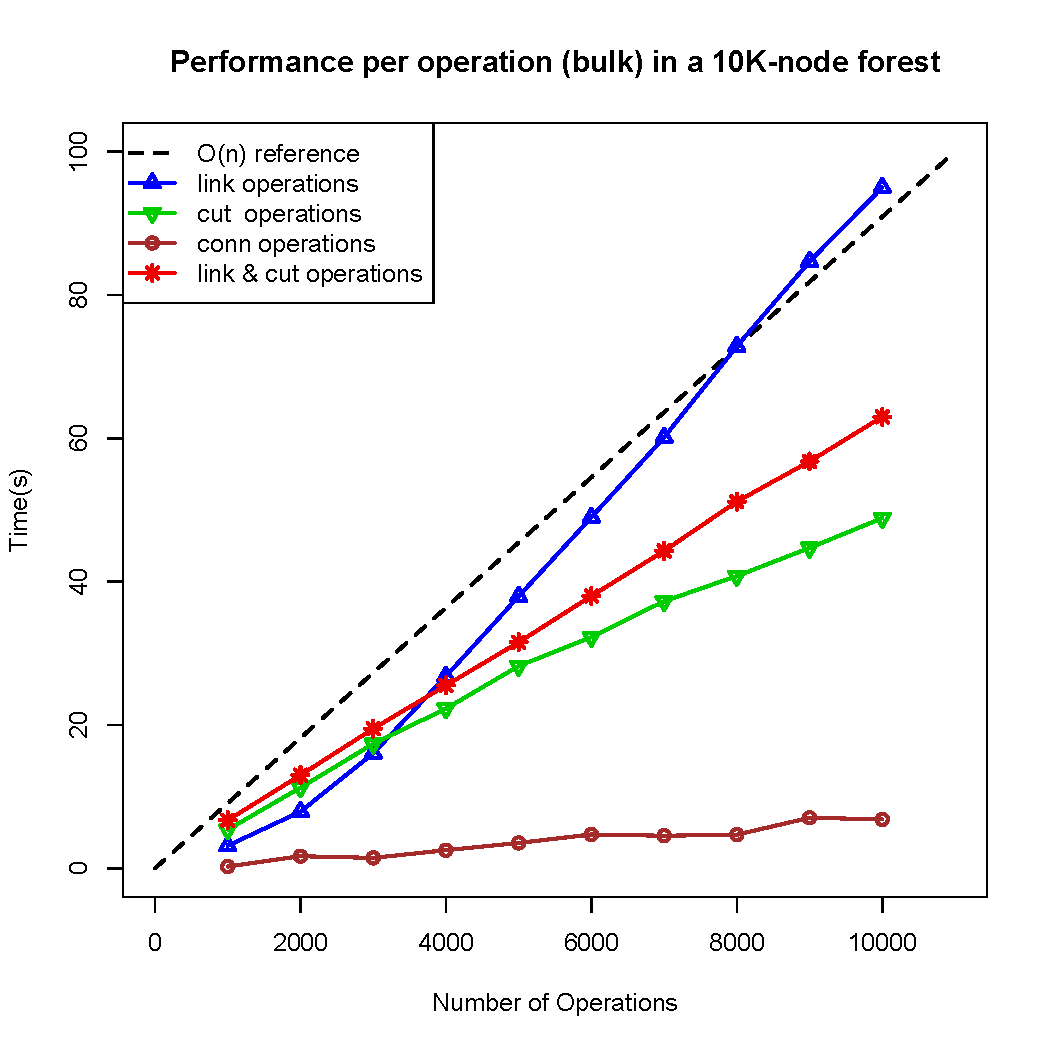
\includegraphics[scale=0.38]{./Images/plotEach}
  \caption{In bulk}
%  \label{fig:sub1}
\end{subfigure}%
\begin{subfigure}{.5\textwidth}
  \centering
  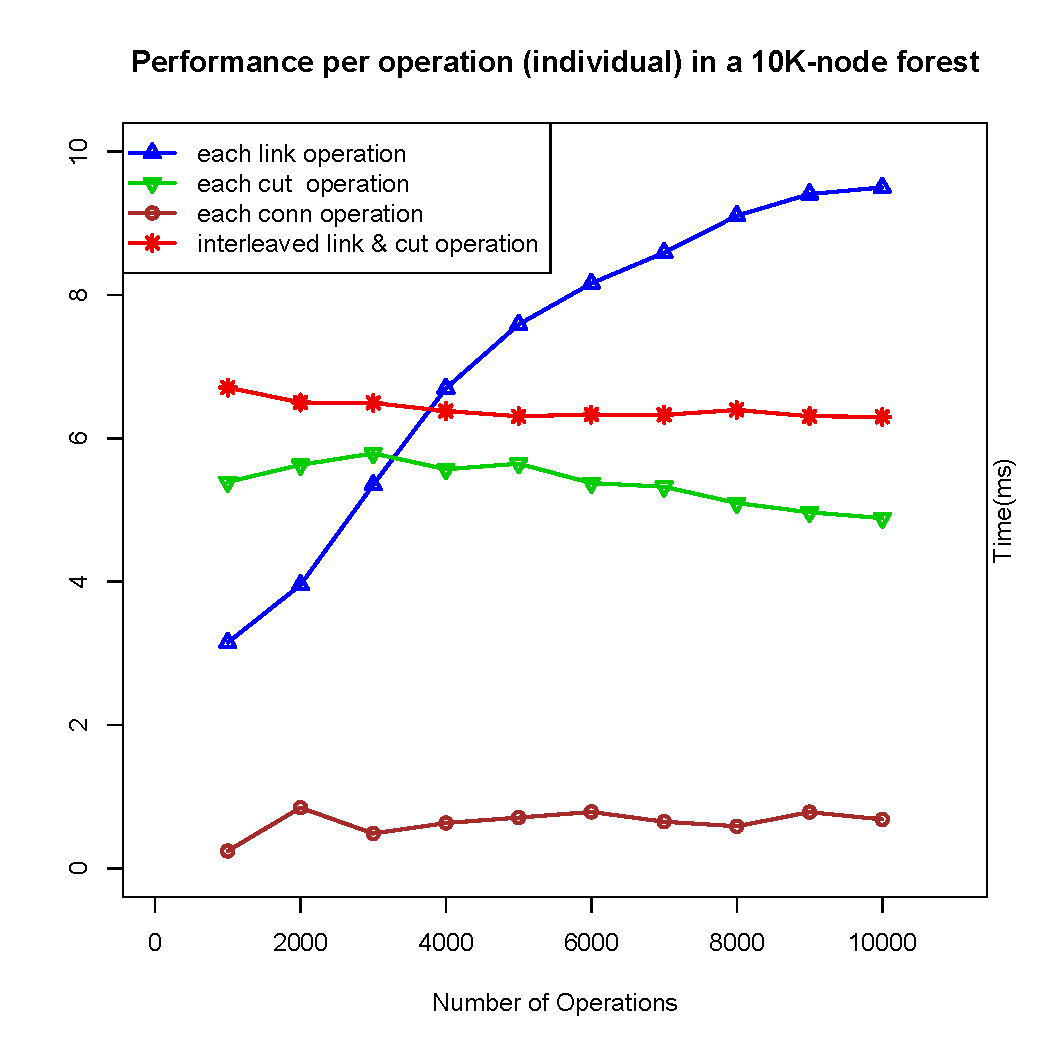
\includegraphics[scale=0.38]{./Images/plotOpsIndiv}
  \caption{Per operation}
%  \label{fig:sub2}
\end{subfigure}
\caption{Time taken by operation, and interleaved \link and \cut}
\label{fig:EachOp}
\end{figure}

\textit{\emph{Results}}. We observe that \cut and \conn obey the same pattern as \link. That is, $\O(1)$ time per operation being \textit{connectivity} the fastest of the dynamic tree operations, as expected.

From the above analyses, we notice that \link performs better when is interleaved with \cut. To see this behaviour closer, we present the bulk and individual cases in the following charts varying the forest size under the same amount of operations.

\begin{figure}[H]
\centering
\begin{subfigure}{.5\textwidth}
  \centering
  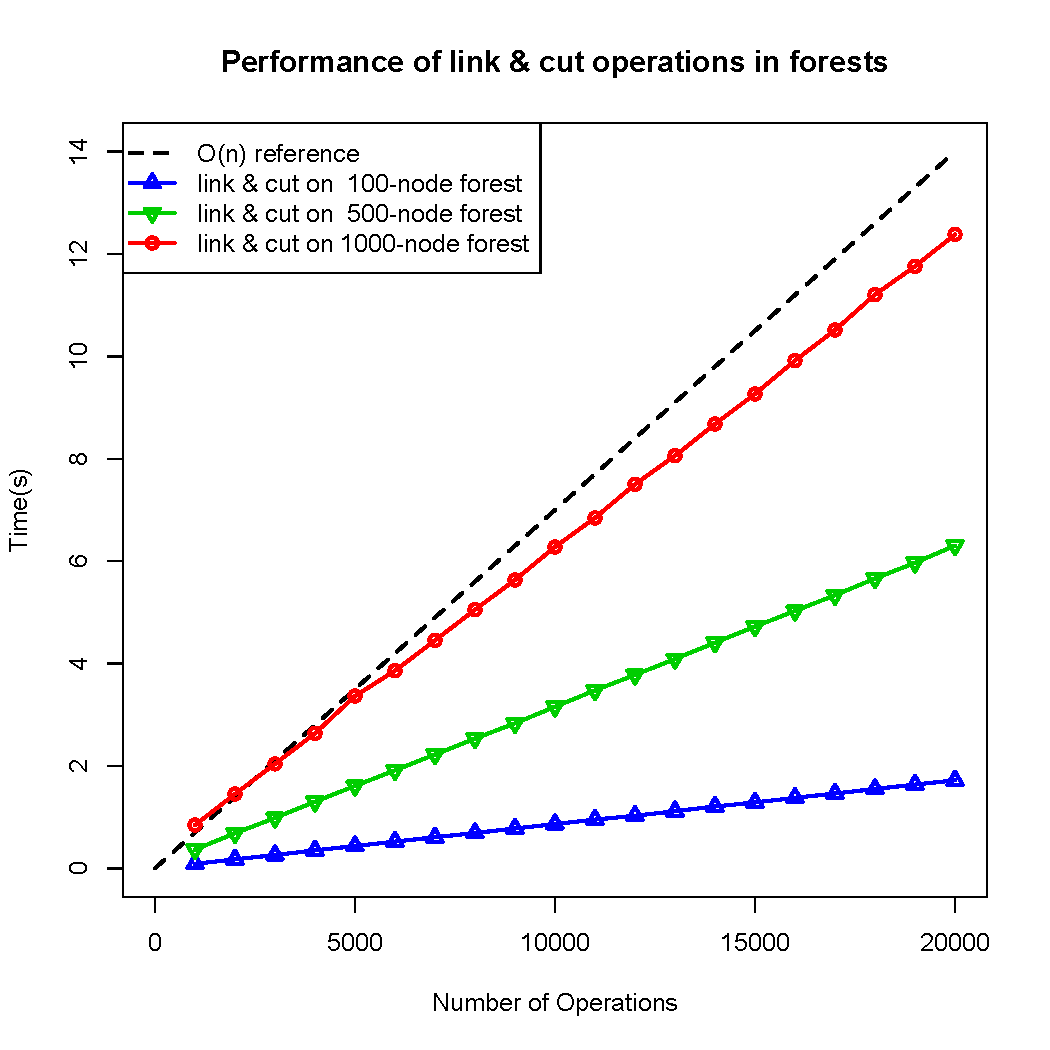
\includegraphics[scale=0.38]{./Images/plotForests}
  \caption{In bulk}
%  \label{fig:sub1}
\end{subfigure}%
\begin{subfigure}{.5\textwidth}
  \centering
  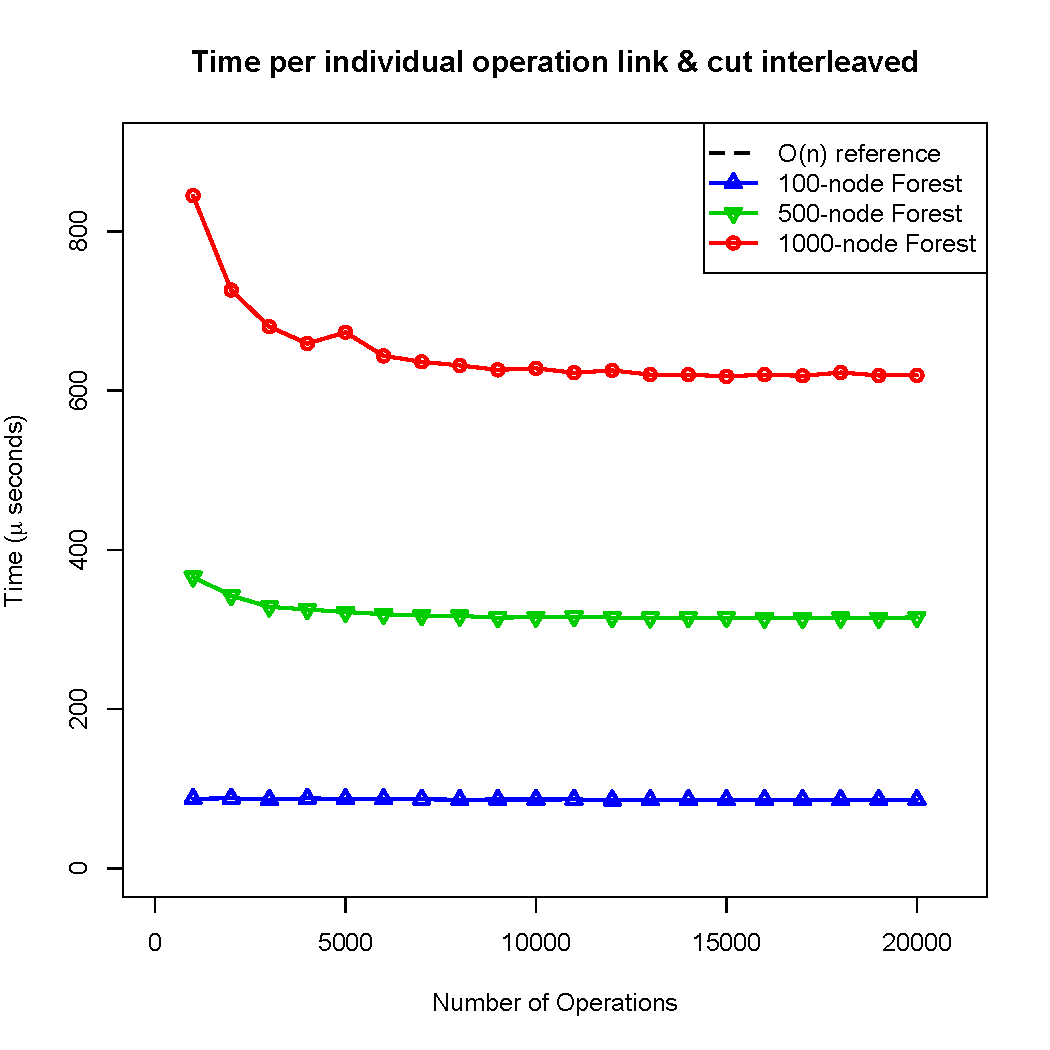
\includegraphics[scale=0.38]{./Images/plotLCForests}
  \caption{Per operation}
%  \label{fig:sub2}
\end{subfigure}
\caption{Time taken when \link and \cut are interleaved with different forest sizes}
\label{fig:EachOp}
\end{figure}

\subsection{Selection of the set data structure}
The set-like data structure is crucial in our implementation and testing of \dyntset since is the search engine for the nodes when any operation is applied to a forest. There are plenty of implementations for such set-like structure, mostly as binary balanced search trees. In our case, where Haskell is a lazy-evaluation language by default, we select two main choices to compare: \code{Data.Set} which is a strict data type definition and \code{Data.Edison.Coll.LazyPairingHeap} which is semi-lazy or semi-strict data type. The following figure shows the performance for each.

\begin{figure}[H]
\begin{center}
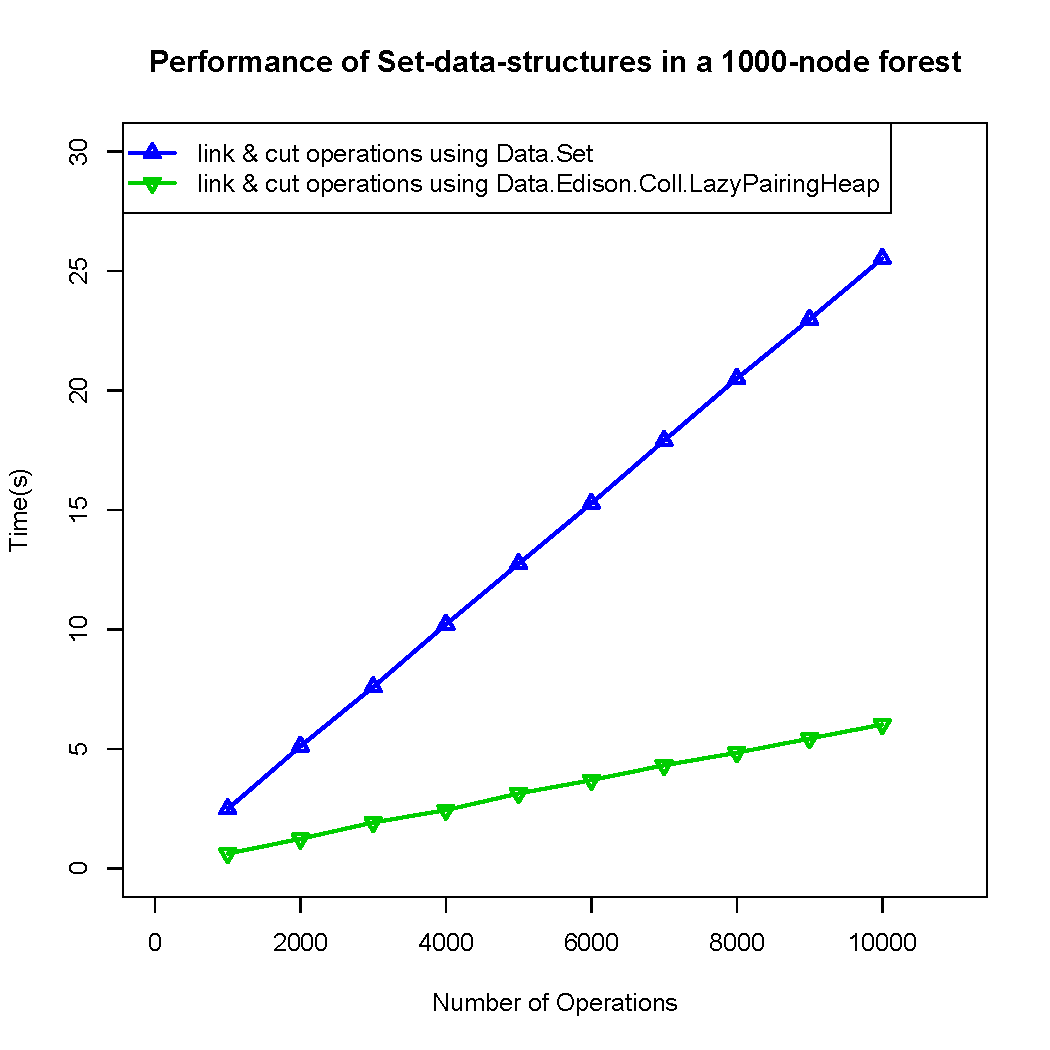
\includegraphics[scale=0.4]{./Images/plotSets} 
\end{center}
\caption{Dynamic operations through different sets structures as monoidal annotations}
\label{fig:plotSets}
\end{figure}

The above curves show that, although by a constant factor, laziness speeds up the running time in the computation of dynamic tree operations through the set-like data structures.

\tcb{Amortised over what??}


%%%% END OF EVAL
%%%% START OF RELWRK

\section{Related Work} 
\label{sec:RelWrk} 

There is a lot of work and research done in the imperative paradigm regarding dynamic tree data structures and related operations. In the other hand, functional programming looks abandoned. In this section we present at least one alternative to finger trees for the Euler-tour trees managed as sequence. Then, we show the current situation about dynamic trees in the Haskell library repository.

\subsection{Functional Sequence}
The Random Access Zipper, or RAZ for short, is an editable sequence within purely-functional data structures. Devised by by Headly and Hammer \cite{RAZ}. The claim here is simplicity, showing the performance between RAZ and finger trees quite closed. The Haskell version for RAZ, provided by Xia \cite{HaskellRAZ}, even implements practically the same operators name for inserting and concatenating elements into the structure such as $\lhd$, $\rhd$ and $\bowtie$ respectively. Apart from the lack of analysis in the performance for the above operators, RAZ does not offer an option for searching access other than an integer index. At this point searching for a specific elements, i.e. the nodes for \link or \cut implies additional interface and implementation.

\subsection{Dynamic trees}

Recall dynamic trees problem can be addressed by three approaches: path decomposition, tree contraction and linearisation. Although our attention was in the latter, through Euler tours, the former can potentially offer a solution for dynamic connectivity, specifically when ignoring the labels over the edges. Kmett \cite{HaskellLC}, provides a Haskell implementation of Link-Cut trees, based on the basic operations defined in Tarjan in \cite{LittleBook}. Although Kmett's basic operations run also in $\O(\log n)$ per operation, his library does not include the forest context so far. 

An additional alternative to linearisation approach is the work done by Moreau \cite{HaskellET}. Also implemented on a finger tree, the monoidal annotation extends our proposal by including a set of nodes and the size of the forest as well as the first and last nodes in the subtrees to allow uniqueness in the edges set.
\begin{lstlisting}[mathescape]
data EulerTourMonoid node = EulerTourMonoid
  (First node)
  (Set (node, node))
  (Last node)
  (Set node)
  (Sum Int)
\end{lstlisting} 

Like Kmett's work, Moreau's implementation also lacks of a forest context definition and interface. Perhaps the major  drawback from Moreau's structure is that of searching. Since every edge in Moreau's finger tree definition is stored only in the monoid and not on the leaves, searching for a specific edge $(x,y)$ trends to return unexpected sub sequences (subtrees), leading to bad formation of Euler-tours hence {\cut}ting and {\link}ing are not accurate.

Finally, Morihata and Matsuzaki \cite{TreeContraction} present a data structure and an algorithm for dealing with tree contraction approach. Nevertheless its computations are described in Haskell, the implementation is done in C\texttt{++}. Their interface does not offer means to perform {\link}s or {\cut}s. The forest context is out of the scope in this publication.

%%%% END OF RELWRK
%%%% START OF CONCL

\section{Discussion and Future Work} 
\label{sec:Concl} 
\label{sec:discussion}

\subsection{Final remarks}

We limit our discussion to dynamic trees. In particular, all data structures we discuss above can solve the dynamic connectivity problem for trees maintaining a forest under a finite sequence of edge insertions and deletions and supporting queries asking whether two vertices belong to the same tree or not.

The experiments we carried out provide a general overview of the strengths and weaknesses of the data structures presented in Sections \ref{sec:TechDes} and \ref{sec:Eval}. Although the results might change slightly if different implementations are tested or if a different architecture is used, some general observations can be made.

Firstly, we have presented \dyntset, a new approach to two existent functional data structures (i.e. finger trees and sets) for maintaining dynamic trees. This structure can manage $k$-degree trees, rooted or unrooted persistently whilst solving the dynamic trees problem. 

Although the updates are conceptually very simple, namely \link and \cut, the proof that both indeed take $\O(\log n)$ time is rather inherited from the core structures. Such definitions are acyclic and involve $\O(1)$ number of steps to perform each. 

Our experimental analysis has shown that the three operations we have implemented exceed the theoretical bounds by a $\O(\log n)$ factor. Also, a native mechanism in the Haskell programming language, the lazy evaluation, is a crucial factor to achieve such performance. Nevertheless, the \link operation is slower that its imperative counterpart, by a factor of $\O(\log n)$, is overcome in practice.

\subsection{Further work}

\tcr{Sets in Haskell are trees themselves, and it is odd to store a tree in every node of a tree. Can you take the finger tree, specialized to this particular monoidal annotation, and optimize it further more?}

Unfortunately, much of the simplicity of \dyntset data structure results from its use of sets as monoidal annotations, which allocate a $\O(\log m)$ space per set within the host structure, i.e. finger tree, where $m \leq n$. Potential improvement suggests that benefits may accrue if we were to use higher order programming with effects, such as stateful computation or database-related structures rather than sets.

Uniqueness on edges allow to carry labels, therefore \dyntset could solve the dynamic trees problem from other approaches such as path-decomposition (i.e. link-cut trees) and tree-contraction. 

Parallelism can play an important speed up when calling functions such \conn. Recalling the its first lines, we have
\begin{lstlisting} [mathescape]
conn x y forest = case (nodeIn x forest, nodeIn y forest) of 
$\ldots$
\end{lstlisting}
Since the result of the leftist \code{nodeIn} is independent from the right one, both are suitable candidates to be evaluated in parallel. The pending research here is the time and space analysis between the sequential (both strict and lazy) against the parallel cases.

Finally, there is an evident need for a library of well-crafted test cases against which implementations of dynamic trees, graphs and applications can be tested. At present, for example, there is little to guide us when generating the update-sequences against which our structures are validated, and this raises a number of obvious issues. For example,

\begin{itemize}
\item Can we find test sets which guarantee coverage of key properties?
\item Which properties are we interested in?
\item If we know the general ratio of updates to queries (say), can we identify a more specific data structure to enhance efficiency still further?
\end{itemize}

These and other questions remain to be addressed, but we believe the quest for efficient dynamic data structures will become ever more important as seek to model, simplify and reason about the increasingly dynamic algorithmic structures in which modern culture is immersed and on which it depends.


%%%% END OF 
%%%% REFS

\bibliography{./Refs/refs}

\end{document}
